\documentclass[11pt]{article}
\usepackage{graphicx} % Required for inserting images
\usepackage{geometry}
\usepackage{float}
\usepackage{array}
\usepackage{booktabs}
\usepackage{amsmath, xparse}
\usepackage{ragged2e}
\usepackage[notes,backend=biber]{biblatex-chicago}
\bibliography{sample}

\geometry{letterpaper, portrait, margin=1in}

\title{Elite orientation of an education system and economic growth}
\author{James Xu}
\date{April 2024}

\begin{document}

\maketitle

\section{Introduction}
Education is a crucial factor in economic development and the progress of countries. Prior literature has found that the mean education level (and the human capital) of a country displays a strong correlation with higher wealth. Mankiw, Romer, and Weil (1992) provided an augmented Solow model where human capital is included as a factor of production. The empirical results support the assertion that education is important in growth. Hanushek and Woessmann (2010) modeled that investments in education which boost PISA scores implies significant gains in GDP. It is widely accepted that the improvement of education in developing countries is a priority with universal primary education being one of the UN Millennium Development Goals.
The allocation of the talented people in a country may provide important economic effects when they work in value-generating positions (i.e. entrepreneurship) versus rent-seeking ones (Murphy et. al., 1991). Within specific industries, the development of technology has allowed superstars to dominate financially at the expense of more moderate performers (Rosen 1981). There are clear economic effects from talented individuals at a country and the same technology which made superstars rich may do the same for countries as well.

However, much of prior research on the macro level has focused on the mean academic achievement. This paper investigates the relationship between the elite orientation of a country’s education system and economic growth. I define “elite orientation” as a composition of cultural and institutional factors which incentives high achievement, competition, and stratification. An education, in this context, is regarded as competition, with actual learning as a side-effect. Conceptually, this is opposed to a “standards-based orientation”, where the goal is to impart knowledge and skill to some specified benchmark.

It is true that an elite-oriented education system may incentive students to engage in competitive behavior and learn skills of dubious practical value. This does not necessarily imply such actions are of no economic value. An economic purpose of acquiring education (beyond the actual “education”) is to signal to employers the capability of the employee (Spence 1973). At a macro level, an elite-oriented education system may thus enable higher levels of stratification and provide additional signals and allow for a more efficient labor market. The extent to which this may relate back to economic growth is a central concern of this paper.

Outside student achievement, the presence of high-performing research institutions may also have a positive effect on economic development. Tertiary education is found to not only have private benefits to individuals, but also more widely for countries (Bloom et al., 2013). More universities per capita are also associated with higher GDP per capita growth (Valero and Van Reenen, 2019). Prior research on this matter has been concerned with simple counts without considering quality.

Measuring the “elite orientation” is not trivial as it is a multidimensional attribute. This paper attempts to measure this using population-adjusted International Math Olympiad test scores, population-adjusted counts of top-ranked universities, and the share of a country’s (or region’s) students testing in the PISA top 1\% for mathematics. The rationale for including these variables as measures of elite orientation are as follows:

\textit{IMO Scores} are included as it reflects the ability for a country/region to develop and identify pinnacle STEM talent at the high school level. Specifically, seeing as the competition involves selecting the 6 best students, the country performance reflects the quality of this selection. Krishna and Haglund (2008) introduced the concept of the effectively participating population which accounts for the fact that not everyone has equal access or interest to sports. This theory was found to be relevant for the IMO as well (Henseke 2009).  In the context of the IMO, after controlling for average education level (equal access), the remaining factor will consist of the level of interest. This level of interest is critical because some incentive outside of being an IMO team member must be available to incentivize the population of students to invest the effort to prepare with the hopes of becoming a team member. The unobservable incentive structures are what we hope to measure with this variable.

\textit{ARWU rankings} are included as it represents the number of elite research institutions a country has. The intent is for this to serve as a proxy for the competitiveness of higher education (ARWU institutions tend to have higher admission standards for undergraduate and graduate education). At the same time, producing top research may also have benefits for economic growth.

\textit{PISA national share in the global 99th percentile} is included as a measurement of the distribution shape of the PISA results. A higher measurement once controlling for average scores may serve as a proxy for wider academic culture (is there an incentive to do well in school).
These variables (“elite orientation variables”) are then included in panel and yearly growth regression models on GDP per capita growth to examine the relationships present. A set of 89 countries across 7 distinct time periods (2003-2022) are included.

This paper finds that the statistical relationship between elite orientation variables and GDP per capita growth is difficult to pin down. In the panel models, it is found that the population-adjusted ARWU-ranked university count and share of students in a country testing in the top 1\% for PISA math is negatively related to GDP per capita growth. However, the population-adjusted IMO score is found to have a positive relationship with GDP per capita growth. While these findings are generally true when looking at individual years, there is significant variation between different years in coefficient direction and magnitude.

Further analysis using PCA suggests that IMO scores capture separate latent factors from the population-adjusted ARWU-ranked university count and share of students in a country testing in the top 1\% for PISA math.

Moretti (2004) found a positive spillover effect exists at the city level where an increase in the number of college graduates increases the wages of non-college graduates. While that study used a fixed-effects model to remove city-specific factors, this paper is aiming to pin down specifically whether an elite orientation is within these fixed effects. The results here suggest that the findings are limited by the data available and there is some potential omitted variable bias on the results.

My results here display a significant difference between models with and without country fixed effects. This is likely due to the elite orientation variables measuring static factors with yearly variations being more idiosyncratic for the most part. Research on explaining IMO scores has found that explaining year-to-year variation is difficult (Henseke 2009).
The remainder of this paper discusses the data used in more detail, the empirical strategy used, and finally the results and limitations of this paper.

\section{Data}
To investigate the central question of the relationship between elite academic performance and GDP per capita growth, I combined national-level data through 2003-2022 from World Bank: World Development Indicators, the Academic Ranking of World Universities (ARWU), PISA test data, the Economist Intelligence Unit Democracy Index, and International Math Olympiad performance results.

The target year range is limited by ARWU ranking data, which is only available from 2003 onwards, and PISA testing data, which is every 3 years (testing in 2021 was delayed to 2022).

In the aggregated dataset, 89 countries are present. Since this is a subset of countries for which PISA test results are available, these countries are wealthier than average. However, there is still a wide range of countries analyzed. Summary statistics are described in table \ref{table:summary}.

\begin{table}
        \caption{Summary Statistics}
        \resizebox{\linewidth}{!} {
            \begin{tabular}{lrrrrr}
                & Count & Mean & Std & Min & Max \\
                \\[-1.8ex]\hline
                \hline \\[-1.8ex]
               GDP per capita & 441.00 & 28463.99 & 25255.10 & 543.11 & 149461.79 \\
               GDP per capita growth (bps) & 440.00 & 169.06 & 452.68 & -2292.68 & 3303.05 \\
               EIU Democracy Index & 441.00 & 7.25 & 1.77 & 1.93 & 9.93 \\
               Primary Completion & 441.00 & 90.00 & 10.25 & 51.35 & 101.95 \\
               Lower Sec. Completion & 441.00 & 77.89 & 17.14 & 29.21 & 101.97 \\
               Upper Sec. Completion & 441.00 & 62.20 & 18.48 & 18.44 & 97.40 \\
               Population & 441.00 & 35318600.19 & 59445620.16 & 34000.00 & 333287557.00 \\
               ARWU per million pop ranked & 441.00 & 0.26 & 0.33 & 0.00 & 1.54 \\
               IMO score per log pop & 441.00 & 4.72 & 3.49 & 0.00 & 11.79 \\
               PISA math in global 1\% & 441.00 & 0.94 & 1.46 & 0.00 & 14.64 \\
               PISA math & 441.00 & 461.93 & 56.23 & 315.96 & 574.66 \\
               \end{tabular}
        }
        \label{table:summary}
\end{table}

I discuss below some of the considerations and transformations applied to the datasets.

\subsection{World Bank WDIs}
The World Bank World Development Indicators (WDIs) are ``a compilation of relevant, high-quality, and internationally comparable statistics about global development and the fight against poverty''. GDP per capita, GDP per capita growth rate, population, and cumulative school completion rates (primary, lower secondary, upper secondary) are sourced from the WDIs.
Specifically, GDP per capita is valued in constant 2015 \$USD. This data was sourced from World Bank national accounts data and OECD National Accounts data files.

The GDP per capita growth rate is the growth in current \$USD. I note that the base levels are different from the GDP per capita levels, but this is unlikely to be a major concern as GDP per capita will only be used as a control variable for wealth.

Finally, the school completion rates represent the cumulative completion rate for each school category for residents above the age of 25. For instance, the primary school completion rate represents ``What \% of the population 25+ has completed primary school?''.

There is a significant missing data problem with the school completion rates. This problem is shown below in figure \ref{fig:wdi}.
\begin{figure}
    \caption{Data availablility for WDIs}
    \centering
    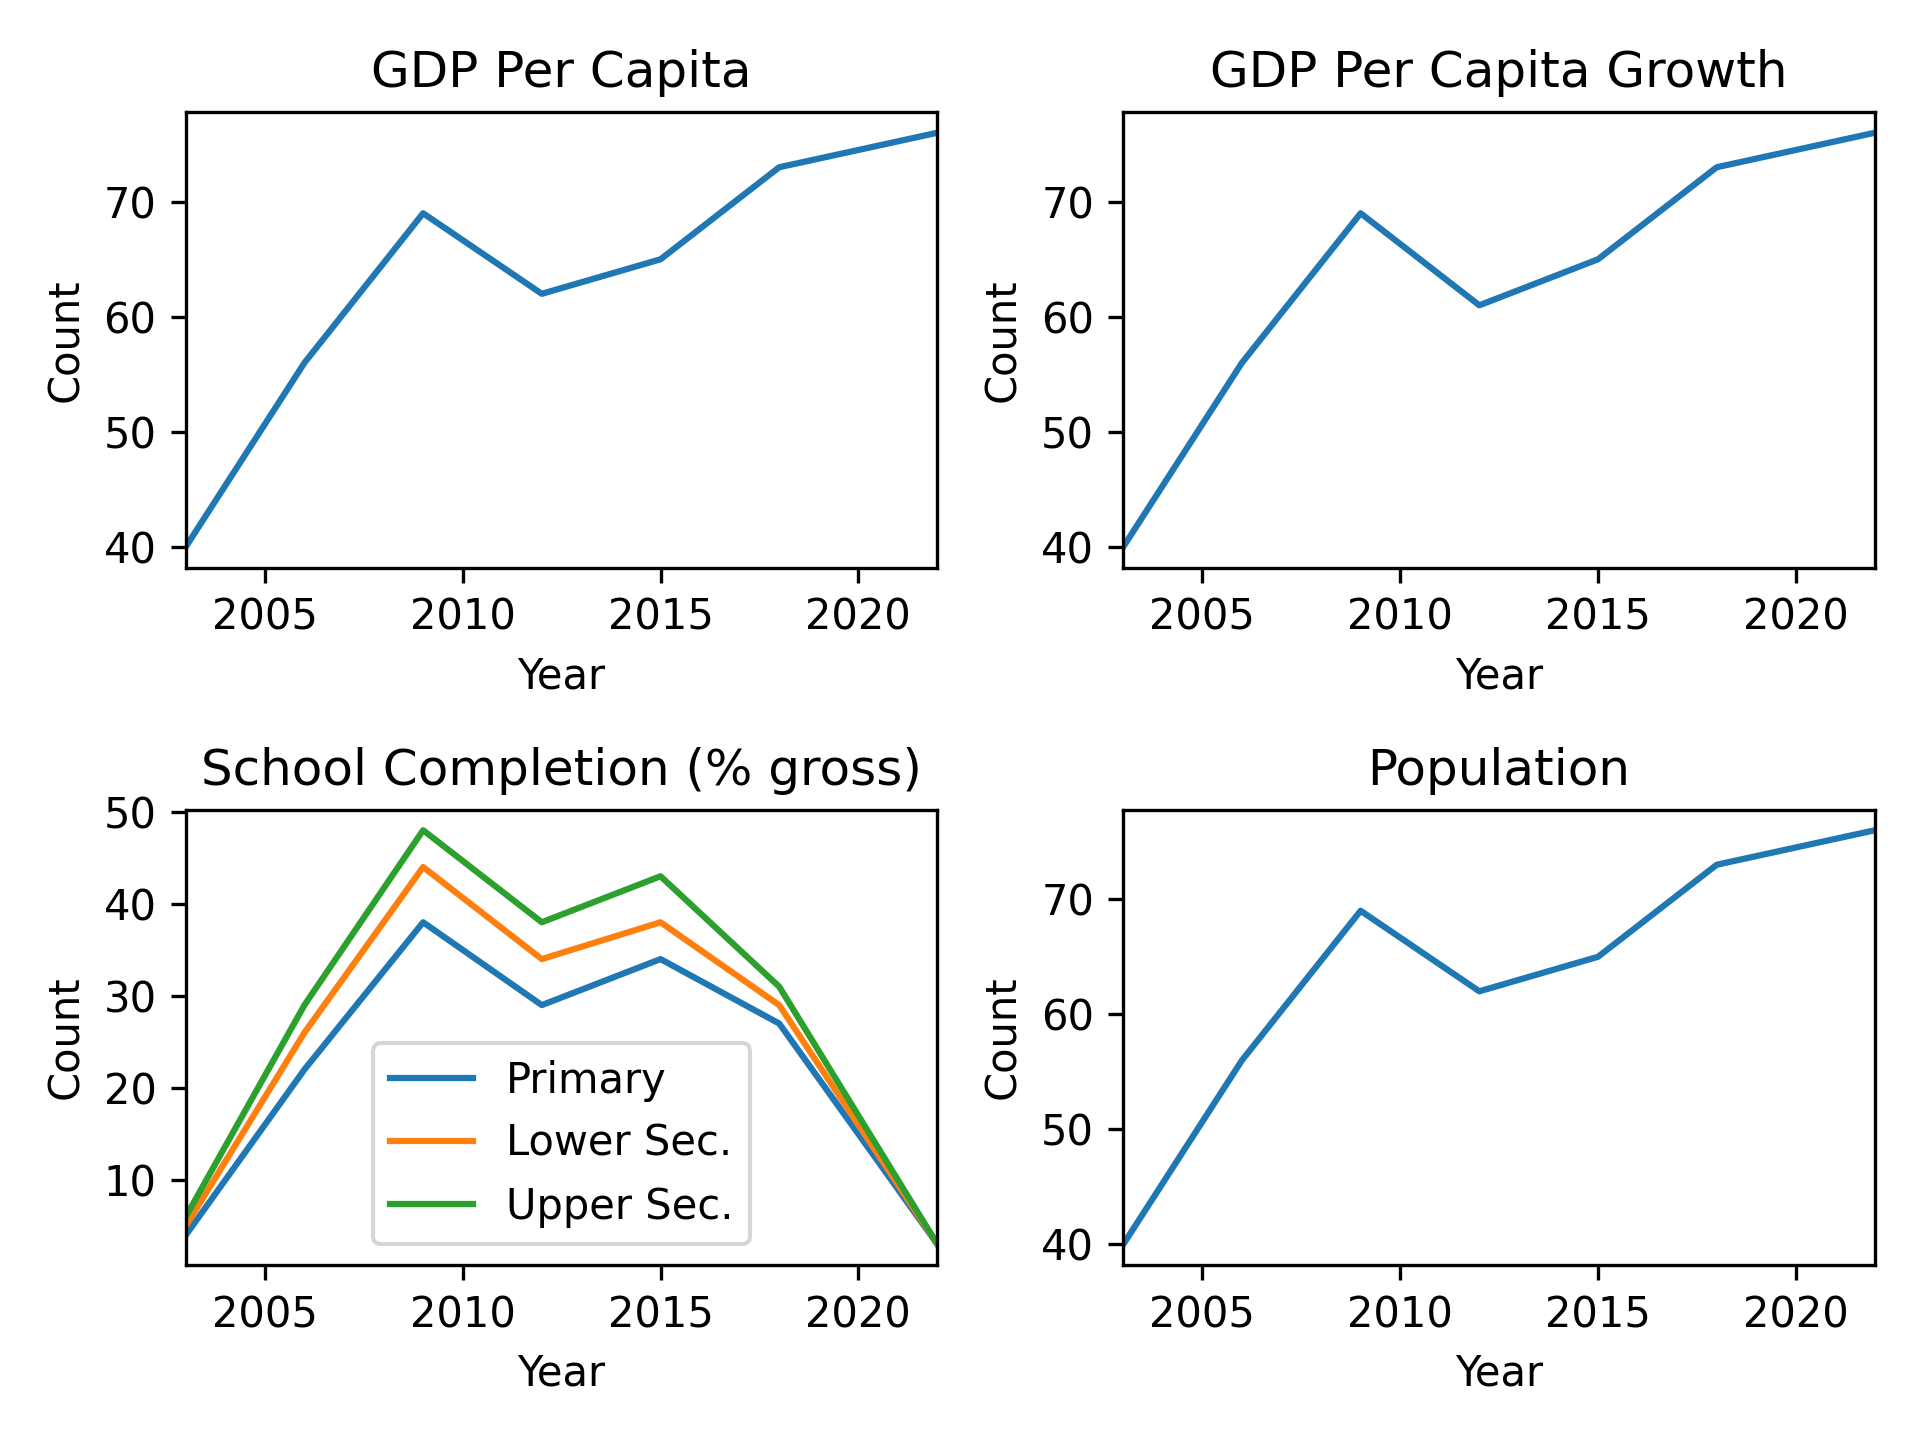
\includegraphics[width=0.6\textwidth]{../charts/wdi-count.png}
    \label{fig:wdi}
\end{figure}

Data for school completion rates are highly limited in the subset of years/countries intersecting with PISA testing. I utilized a custom XGBoost model trained on a superset of the dataset used in this paper to impute nulls. I describe this further below in a separate section.

\subsection{ARWU Rankings}
The ARWU rankings are a set of university rankings produced previously by Shanghai Jiaotong University but by the Shanghai Ranking Consultancy now . ARWU ranks the top 1000 universities (500 before 2017).

Compared to other rankings such as Times Higher Education (THE) and Quacquarelli Symonds (QS), the ARWU rankings are more quantitative, and research focused. A university's score is determined by ``Quality of Education'' (alumni with Nobel and Fields medals), ``Quality of Faculty'' (faculty Nobel and Fields medal, highly), ``Research Output'' (Nature/Science publications, top social science papers), and ``Per Capita Performance''\footnote{This was retrieved from https://www.shanghairanking.com/methodology/arwu/2023}.

For each country and year, the total number of ranked of universities is calculated. Finally, the counts are transformed as follows into a per million population metrics.
\begin{equation}
    ARWU_{i,t} = \frac{arwuCount_{i,t}}{P_{i,t}} \cdot 10^6
\end{equation}
Prior research by Valero and Reenen (2019) has also used a per-capita measure in growth regressions. Some limitations to this measure are that it does not consider university size or the quality of it beyond it merely being ranked.
\subsection{PISA Scores}
PISA, or Programme for International Student Assessment, is an assessment of student achievement where 15-year-old students are tested. As it is a sample-based estimation of student achievement, the dataset includes student weights that must be incorporated when taking aggregates.
\begin{equation}
    math_{c, t} = \frac{\sum_{i \in c \cap t} stu\_math_i \cdot stu\_wgt_i}{\sum_{i \in c \cap t} stu\_wgt_i} \\
\end{equation}
Another consideration is the use of plausible values in the PISA data set. Data from 2003-2018 is sourced from the Leaning Tower dataset\footnote{https://kevinwang09.github.io/learningtower/index.html} while the 2022 data is sourced directly from PISA. In 2022, the plausible values were not computed per specification but only taken together to compute a mean math score. Only the math score was used to make the regression easier to interpret.

A measure of ``elite orientation'' is created by computing the share of students in a given country and year scoring above the top 1\% cutoff line in that year.

\begin{equation}
    math99_{c, t} = \frac{\sum_{i \in c \cap t} (stu\_math_i \geq B_t) \cdot stu\_wgt_i}{\sum_{i \in c \cap t} stu\_wgt_i}
\end{equation}

\subsection{IMO Scores}
I collected the IMO scores per country for each year from 2003-2022 from the IMO website. Each country may send a maximum of six students and there are 6 questions, each out of 7 points. A total of 252 is the maximum possible score.

Previous literature discussing Olympic medals have found a positive relationship with log population (Krishna and Haglund, 2008). This is due to the talent pool benefits a larger country experience. For instance, China may have 1-2 “1 in a billion” talent (can be solving math problems or doing long jumps), but a small country like Singapore with a population of 5 million will not likely have this. While a different competition, the premise and logistics of the IMO and the actual Olympics are highly similar. Thus, I correct for this in my paper by dividing the IMO scores by the log population. This is done by applying transformation $t(s)$ to each score:
\begin{equation}
    t(s) = \frac{s}{\log P}
\end{equation}
This should remove the effect of population in the talent pool from this variable so it may reflect more purely relative performance.

\subsection{EIU Democracy Index}
The Economist Intelligence Unit publishes annual qualitative rankings of democracy around the world for 160+ countries and territories/regions. Ratings are assigned from 0-10, with 0 being a pure dictatorship/autocracy and 10 being democracy. The index was first published in 2006 every 2 years until 2010, but it is now published annually. Nulls in the years not included were imputed using an XGBoost model discussed below. Please see figure~\ref{fig:eiu} for a snapshot

This helps control for style of governance and quality of governance institutions. The measurement is qualitative. Prior research has shown importance of good policies and governance and I discuss potential correlations with IMO scores further in the empirical strategy section (Burnside and Dollar, 2000).

\begin{figure}[H]
    \caption{Index scores in 2023}
    \centering
    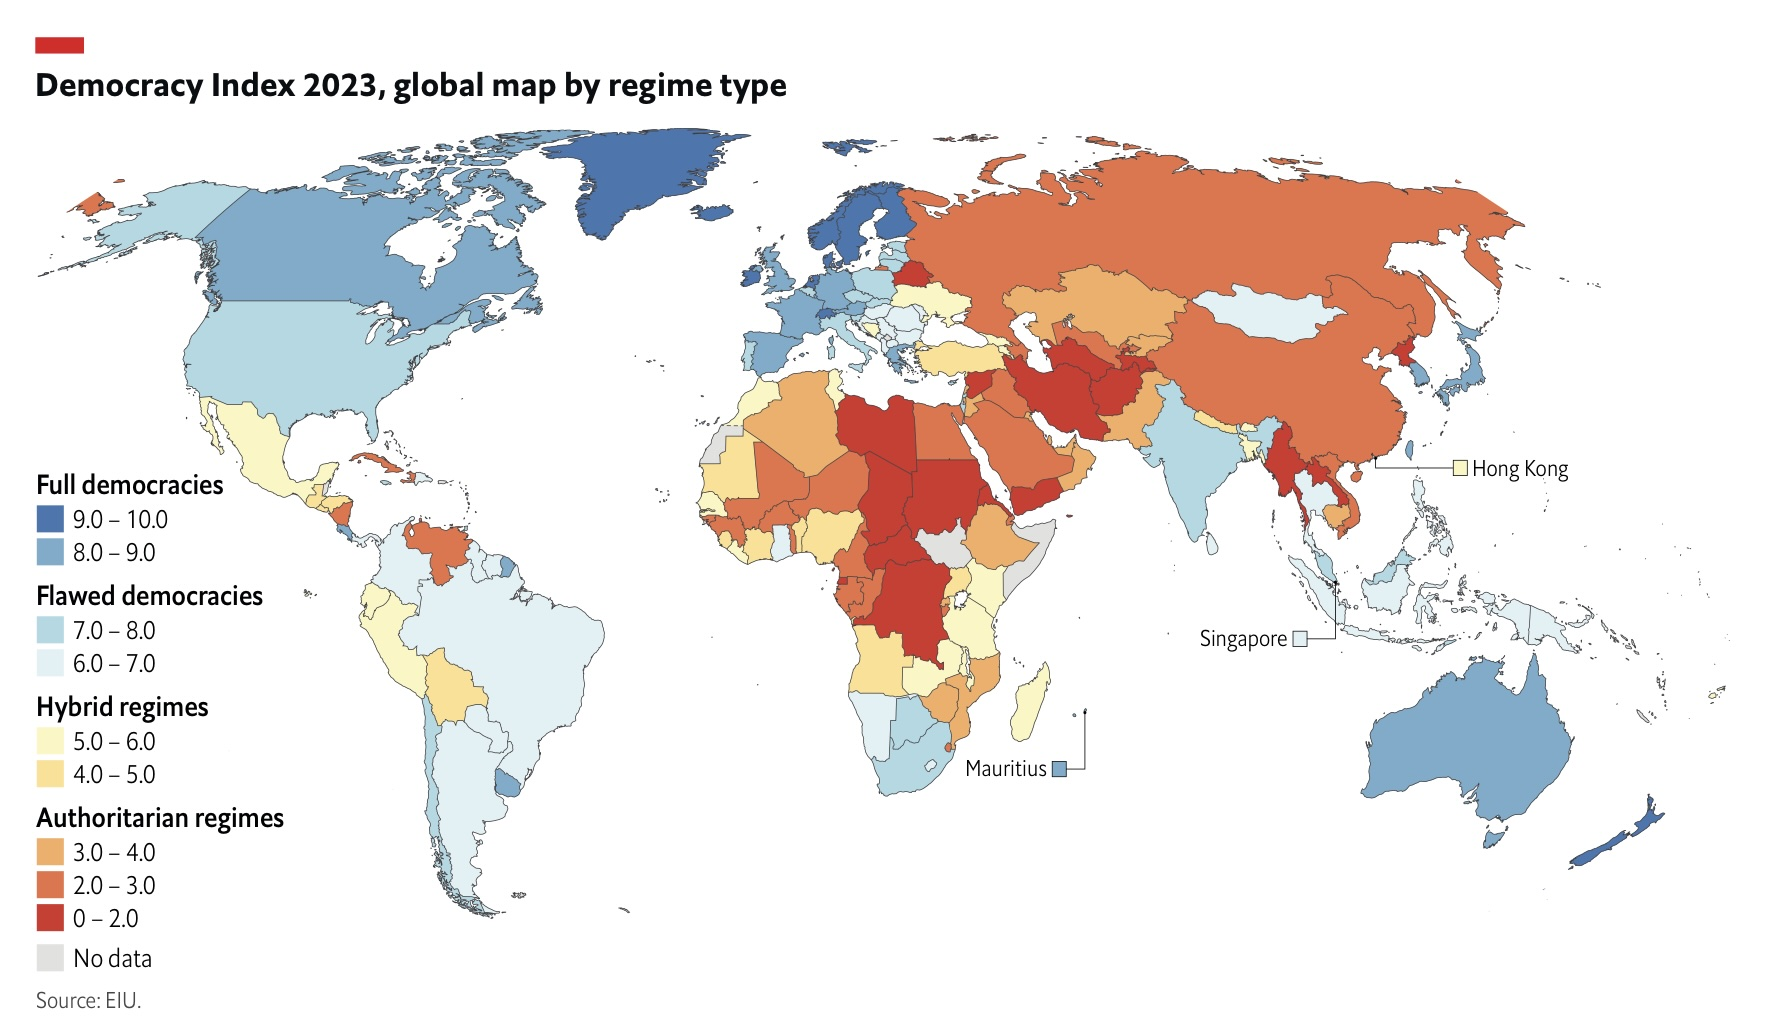
\includegraphics[width=0.6\textwidth]{../charts/eiu_2023.jpg}
    \label{fig:eiu}
\end{figure}
\subsection{XGBoost Imputation}
Missing data is a significant problem for the school completion rates and the EIU Democracy Index (not collected in several PISA years). I used XGBoost, a gradient-boosted tree model, to train a prediction model for school completion rates and democracy index.

The training dataset consists of annual data from 2003-2022 using the following variables:
\begin{itemize}
    \item GDP Per Capita
    \item EIU Democracy Index (country mean for EIU Democracy Index model)
    \item School Completion Rates (not included for that model)
    \item PISA math mean
    \item IMO score per log population
    \item ARWU-ranked universities per million population
\end{itemize}

XGBoost can intelligently handle nulls, which is why all the variables were included to optimize accuracy. A 70/30 train-test-split was used. GridSearchCV (using 5-fold cross validation) from scikit-learn was used for hyperparameter tuning while optimizing for RMSE. The best fit model for school completion rates achieved an RMSE of 13.52 and an $R^2$ of 0.71 on test data. However, on training data, the $R^2$ is significantly higher at 0.96, indicating some overfitting. Looking at the distributions it appears that XGBoost is underpredicting counts in the highest bucket of completion rates. Please see figure \ref{fig:xgboost-school} for school completion rate results.

\begin{figure}[H]
    \caption{Training results for school completion rates}
    \centering
    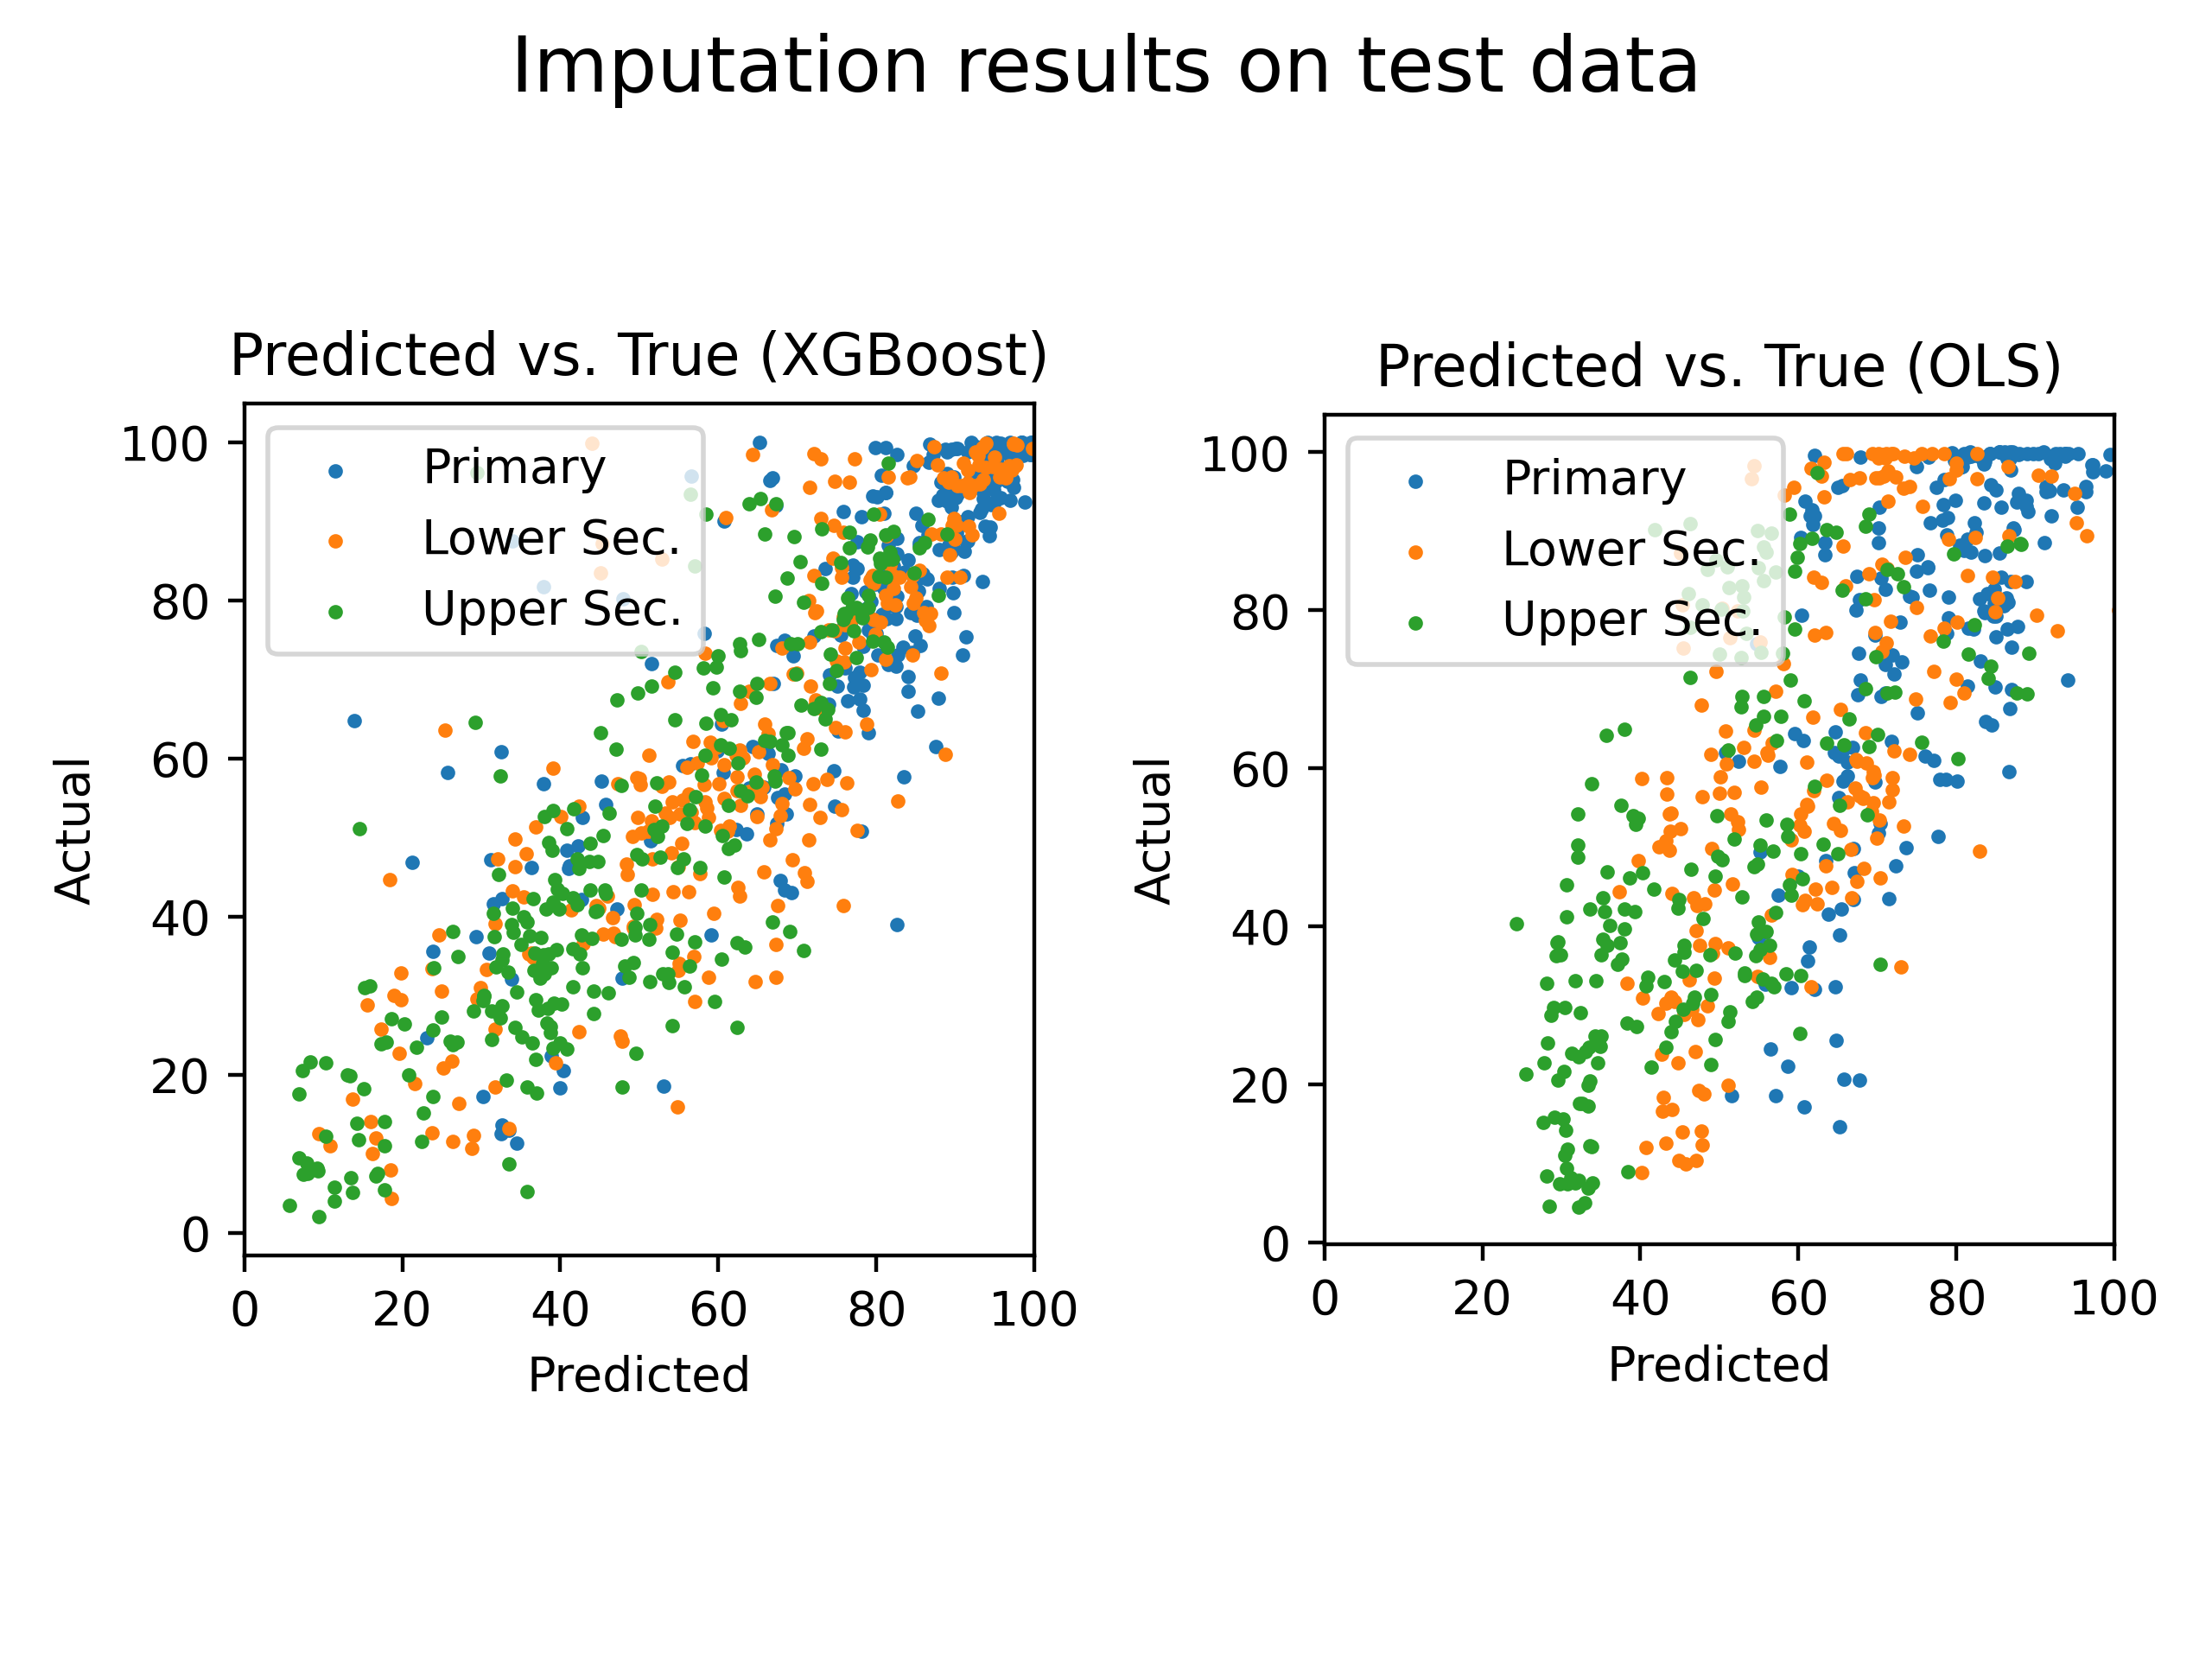
\includegraphics[width=0.6\textwidth]{../build/xgboost.png}
    \label{fig:xgboost-school}
\end{figure}

Results are significantly better for the EIU Democracy Index model data is available for all countries, just not all years. The mean index score for each country is included and this helps the model achieve better results. In this case, the test data $R^2$ is 0.98. An OLS model achieves a similar $R^2$ of 0.96 as the inclusion of the mean is doing the heavy lifting. See figure \ref{fig:xgboost-eiu} for EIU democracy index training results.

\begin{figure}[H]
    \caption{Training results for EIU democracy index}
    \centering
    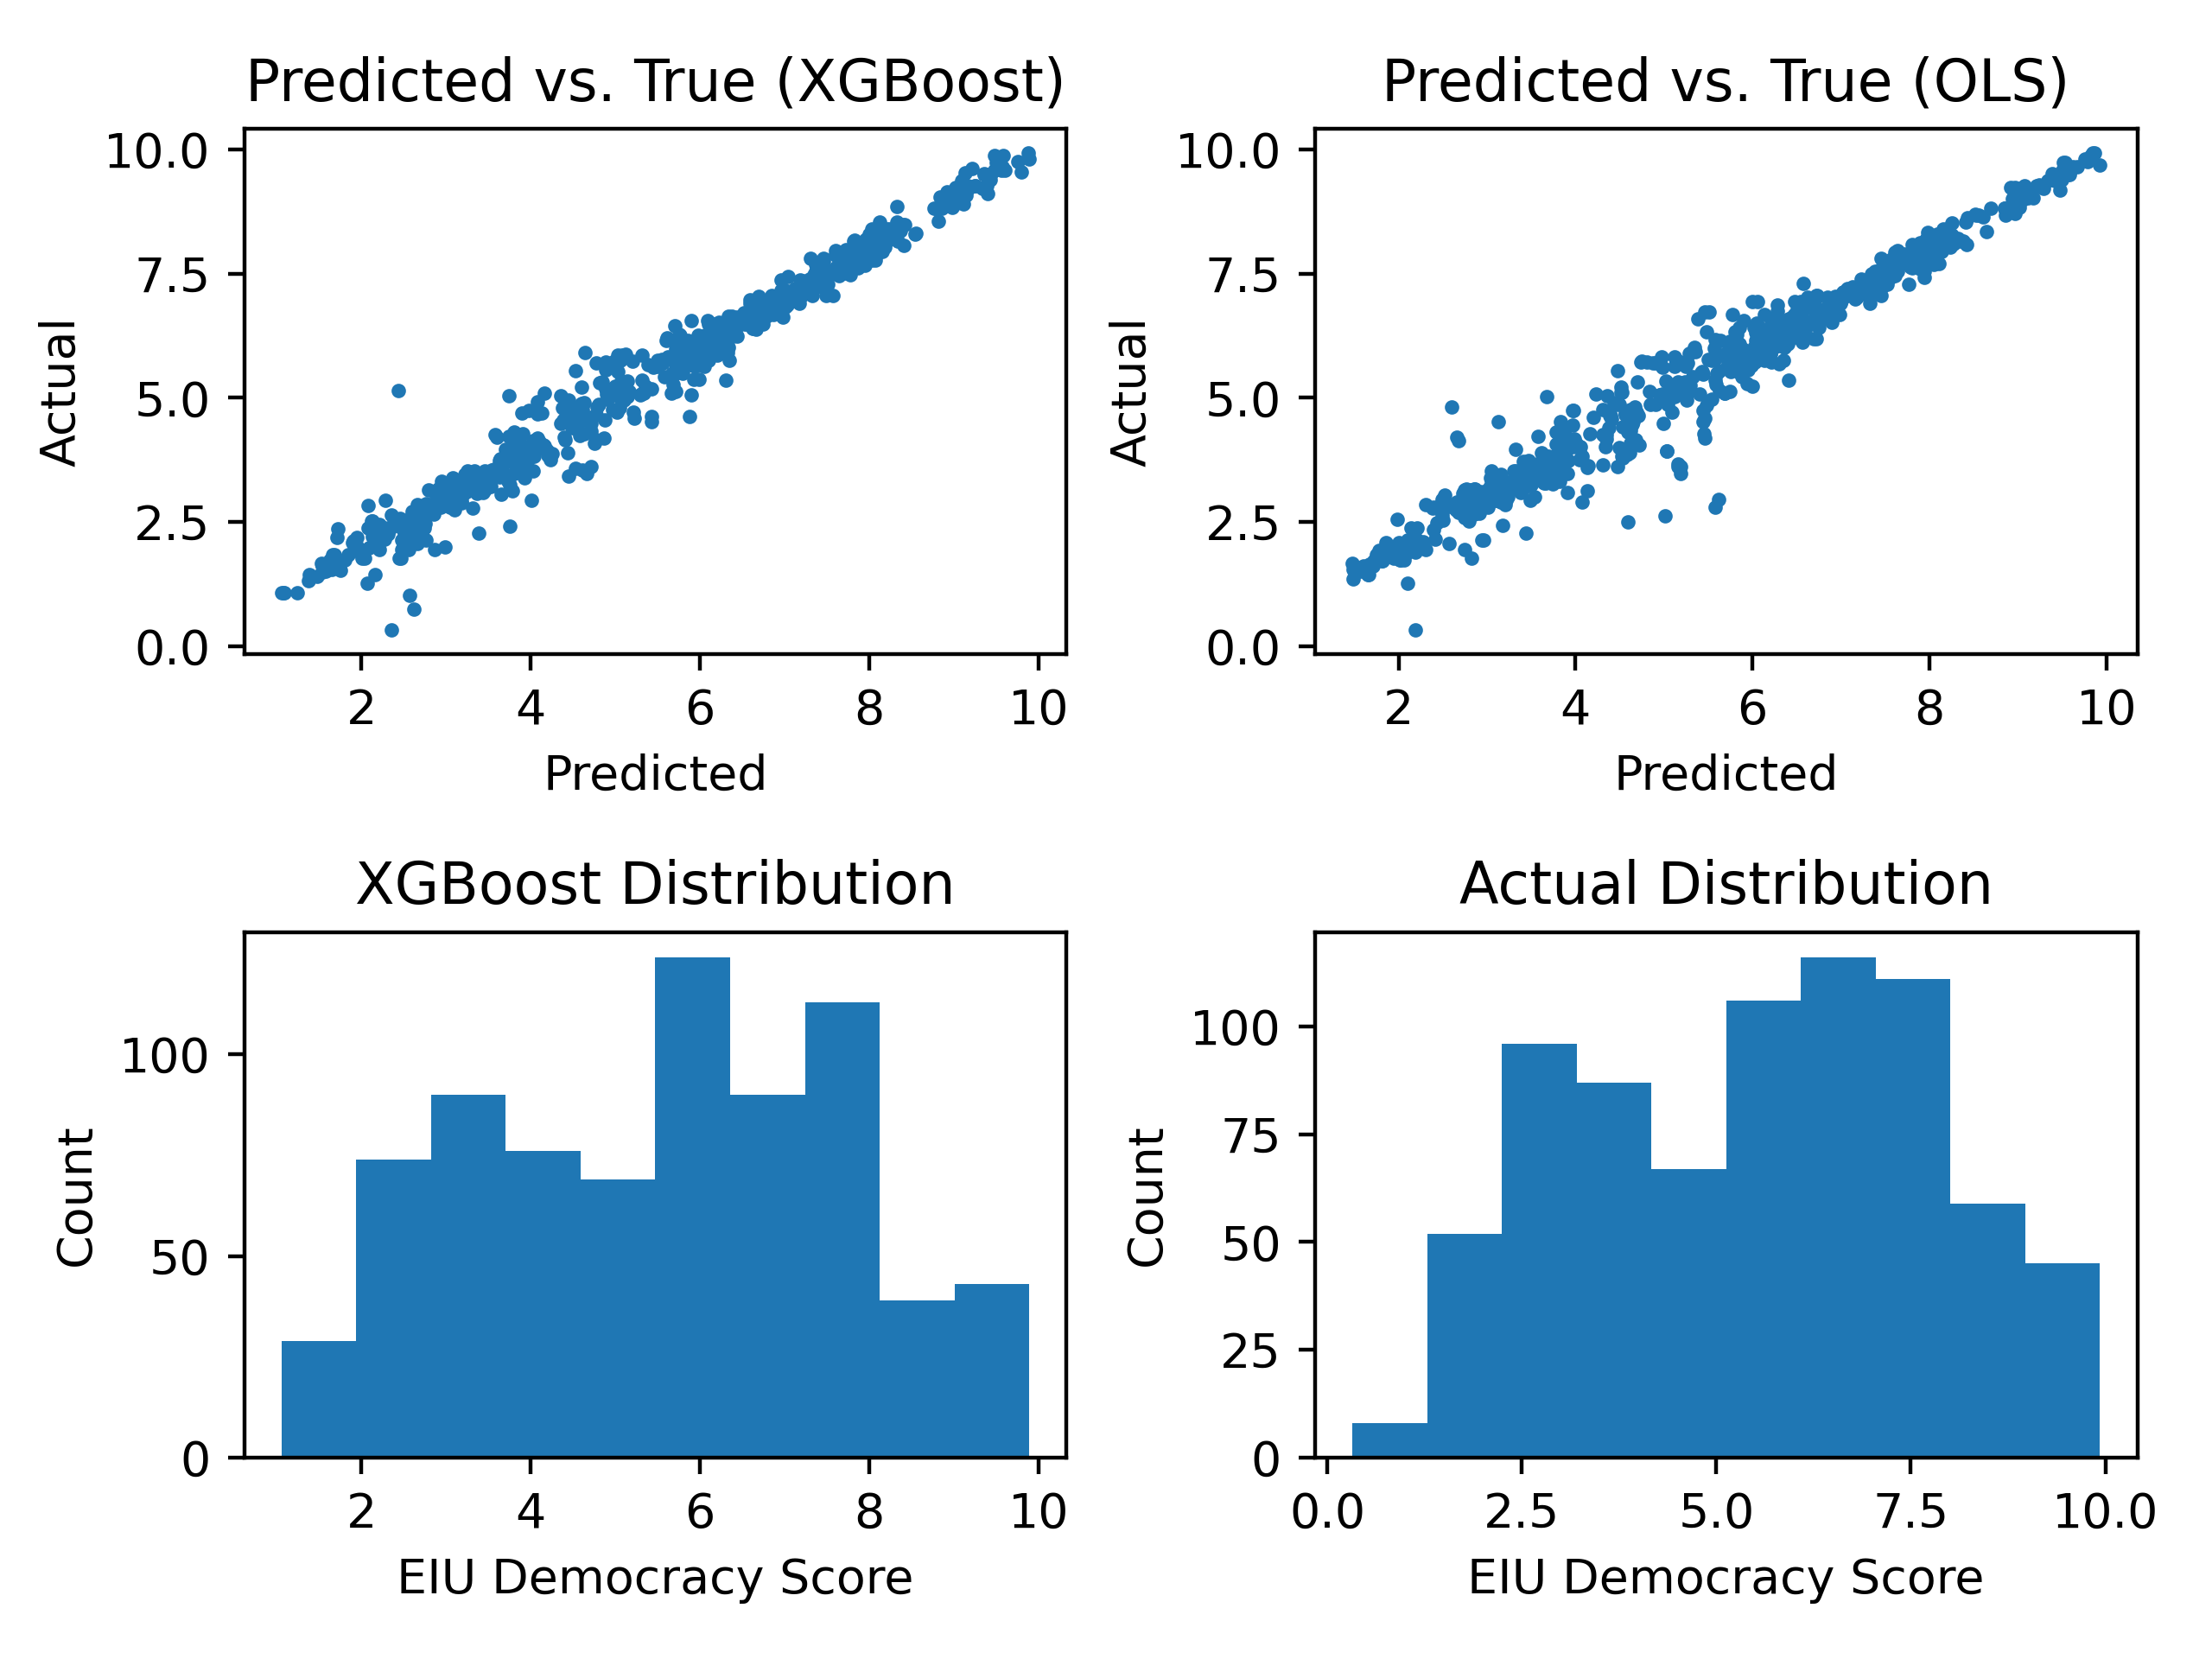
\includegraphics[width=0.6\textwidth]{../build/eiu_xgboost.png}
    \label{fig:xgboost-eiu}
\end{figure}
\subsection{Trends in data}
For the three elite orientation variables, they are mostly stable through time within countries. Consequently, most of the variation present is between countries. Please see figure \ref{fig:trends} for a year-by-year breakdown.
\begin{figure}[H]
    \caption{Trends in elite orientation variables over time}
    \centering
    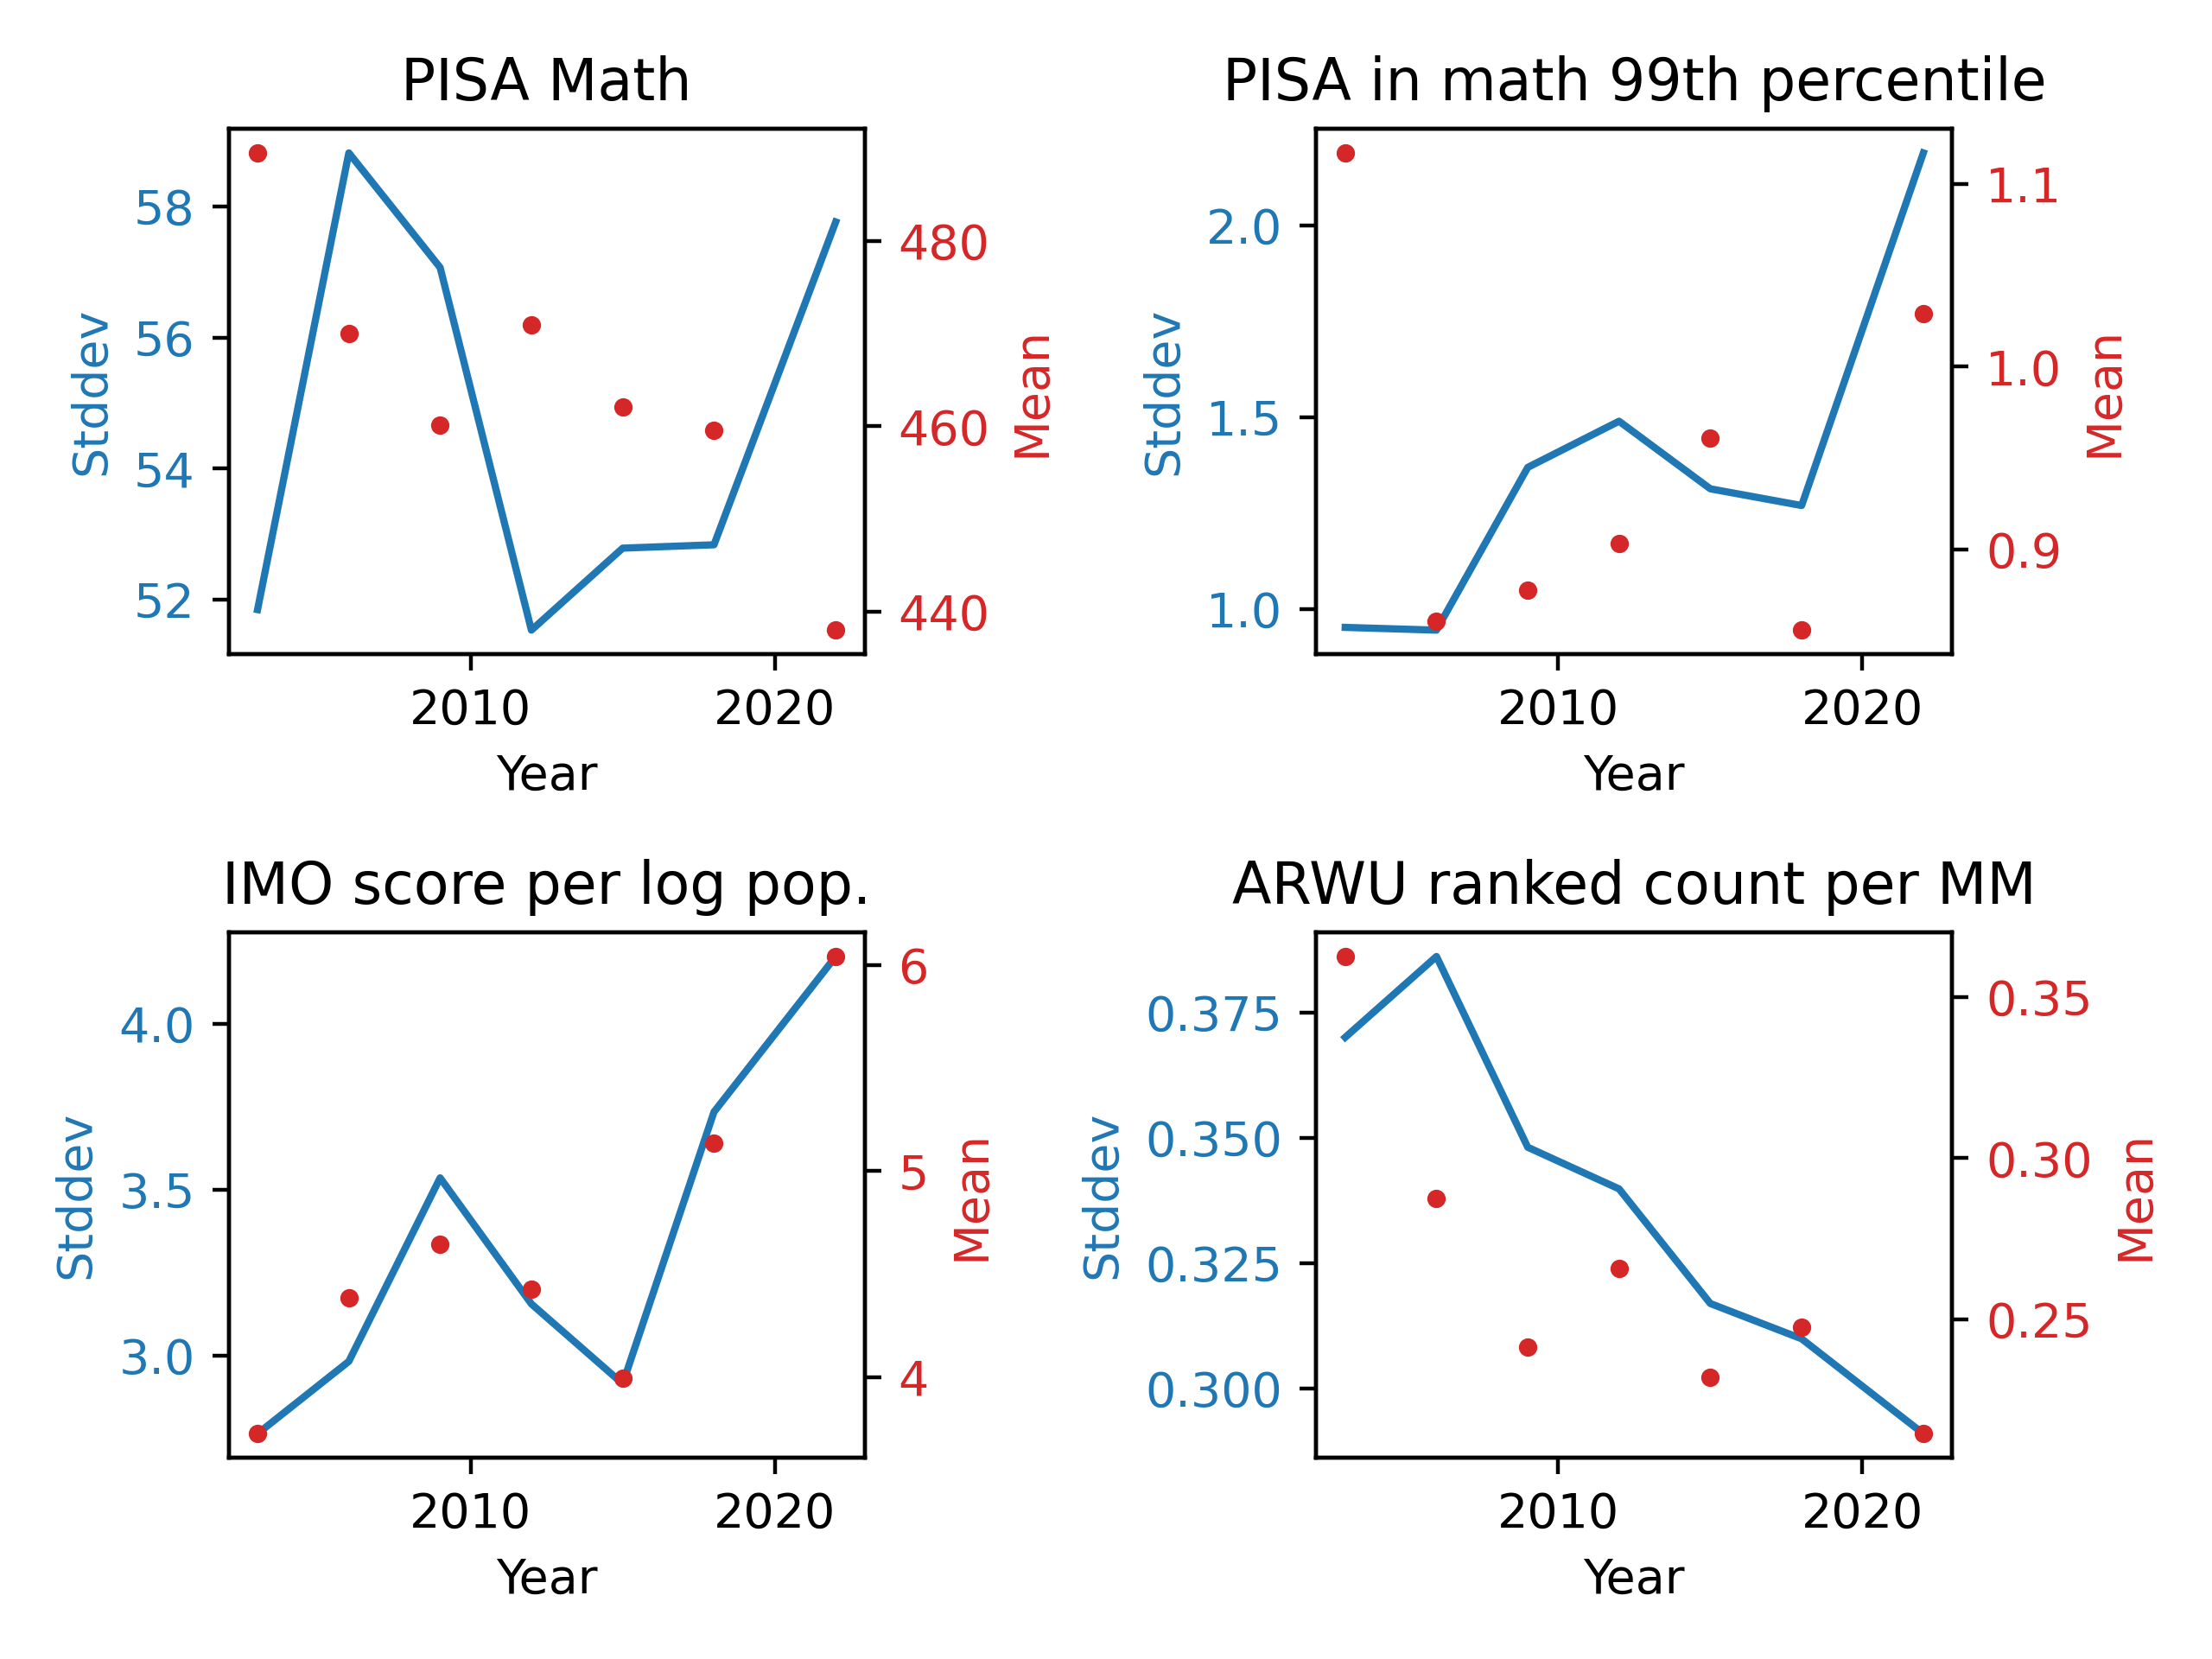
\includegraphics[width=0.6\textwidth]{../charts/std-dev.png}
    \label{fig:trends}
\end{figure}

In the period of consideration (2003-2022), the average PISA math test score has been decreasing while the per-year standard deviation has remained steady. Math education quality has diverged rather than converged while overall ability has decreased.

This picture is made clearer by looking at PISA math 99. The within-year standard deviation has steadily increased from 2003 while the mean has increased. Globally, higher-performing countries are claiming a higher share of the best-performing students, painting another picture of educational divergence.

Conversely, for the number of ARWU-ranked universities per million, the situation is instead of convergence. Since the rankings are ``zero sum'', this is likely driven by the increasing research output and quality of universities outside the U.S. and western Europe.

Average IMO scores have also gradually increased over the years, but this is hard to interpret as it may reflect either achievement or the test becoming easier.

\section{Empirical Strategy}
To investigate the relationship between elite orientation and economic growth, I construct regressions which target GDP per capita growth (converted to basis points) with the elite orientation variables (PISA math share in 99th percentile, IMO score per log population, and the number of ARWU ranked institutions per million population). The following controls are included:

\textit{GDP per capita} is included as a control to address the concern that wealthier countries may have more resources and a better education system which may bias the regression.

\textit{Population} is included to control for any remaining correlation between the elite orientation variables and country size.

\textit{School completion rates} are included to control for a baseline “human capital” measure along with PISA math scores, except this measure corresponds to the whole population rather than just the tested subset (weighting may not be perfect in PISA).

\textit{PISA average math scores} are included to control for a baseline academic achievement level as countries with higher elite orientation variables will generally have better education results and this will help control for that.

\textit{Democracy Index} is included to address concerns that more autocratic countries may have a higher elite leaning, especially as it reflects on IMO scores. The IMO originated as a Communist bloc event with the first event consisting of Romania, Hungary, Czechoslovakia, Bulgaria, Poland, the USSR, and the GDR\footnote{See 1959 IMO participating countries}.

The relationship between the elite orientation of an education system and economic growth is difficult to measure. First, the variables available to measure elite academic performance are related to other unobservable variables which relate to economic growth and development. For instance, cultural attitudes toward education, structural incentives, the fairness of the labor markets, even the fairness of education systems, are likely to be related to both.

Second, it is not necessarily true that the relationships are static over time or changing. I have no reason to suspect one over the other a priori, so I construct two sets of regressions to analyze this further.

\subsection{Panel Regression}
Assumes the relationship is the same between countries and between years. I also test different specifications with time and country fixed effects. Adding country fixed effects restricts this to be a within regression, which implicitly assumes that there exists meaningful variation between different years for one country.

Let elite indicators be: $math99, ARWU, IMO$.
For the sake of concision, let $E_{i,t}$ be a 1 by 4 matrix defined as:
\[E_{i,t} = 
\begin{bmatrix}
    math99_{i, t} & ARWU_{i, t} & IMO_{i, t}
\end{bmatrix}
\] for country/region $i$ in year $t$.
For control variables, $I_{i, t}$ is the matrix of variables and $\alpha$ is coefficients.
\begin{equation}
    Y_{i, t} = \beta_0 + \lambda E_{i, t} + \alpha I_{i, t} + T_t + C_i + \epsilon_{i, t}
\end{equation}
where $T,C$ represent time and entity dummies respectively and $Y_{i,t}$ be the GDP per capita growth in basis points for a country/region $i$ and year $t$.
\textbf{Controls: school completion rates, GDP per capita, PISA average math score, democracy index, population.}

\subsection{Yearly Regressions}
Separate regression for each year. Does not make the assumptions above. We modify the equation above to remove fixed effects.
\begin{equation}
    Y_{i, t} = \beta_0 + \lambda E_{i, t} + \alpha I_{i, t} + \epsilon_{i, t}
\end{equation}
\subsection{Interpretion and goals}
This paper does not aim to make any causal inference as it is complicated by omitted variable bias and the reality the elite academic orientation variables are merely instruments for unobservable characteristics. GDP per capita growth obviously has many contributing factors, and so a simple scatter plot (see figure \ref{fig:relationships}) is insufficient at determining whether a statistical relationship exists.
\begin{figure}[H]
    \caption{Relationships of variables with GDP per capita growth}
    \centering
    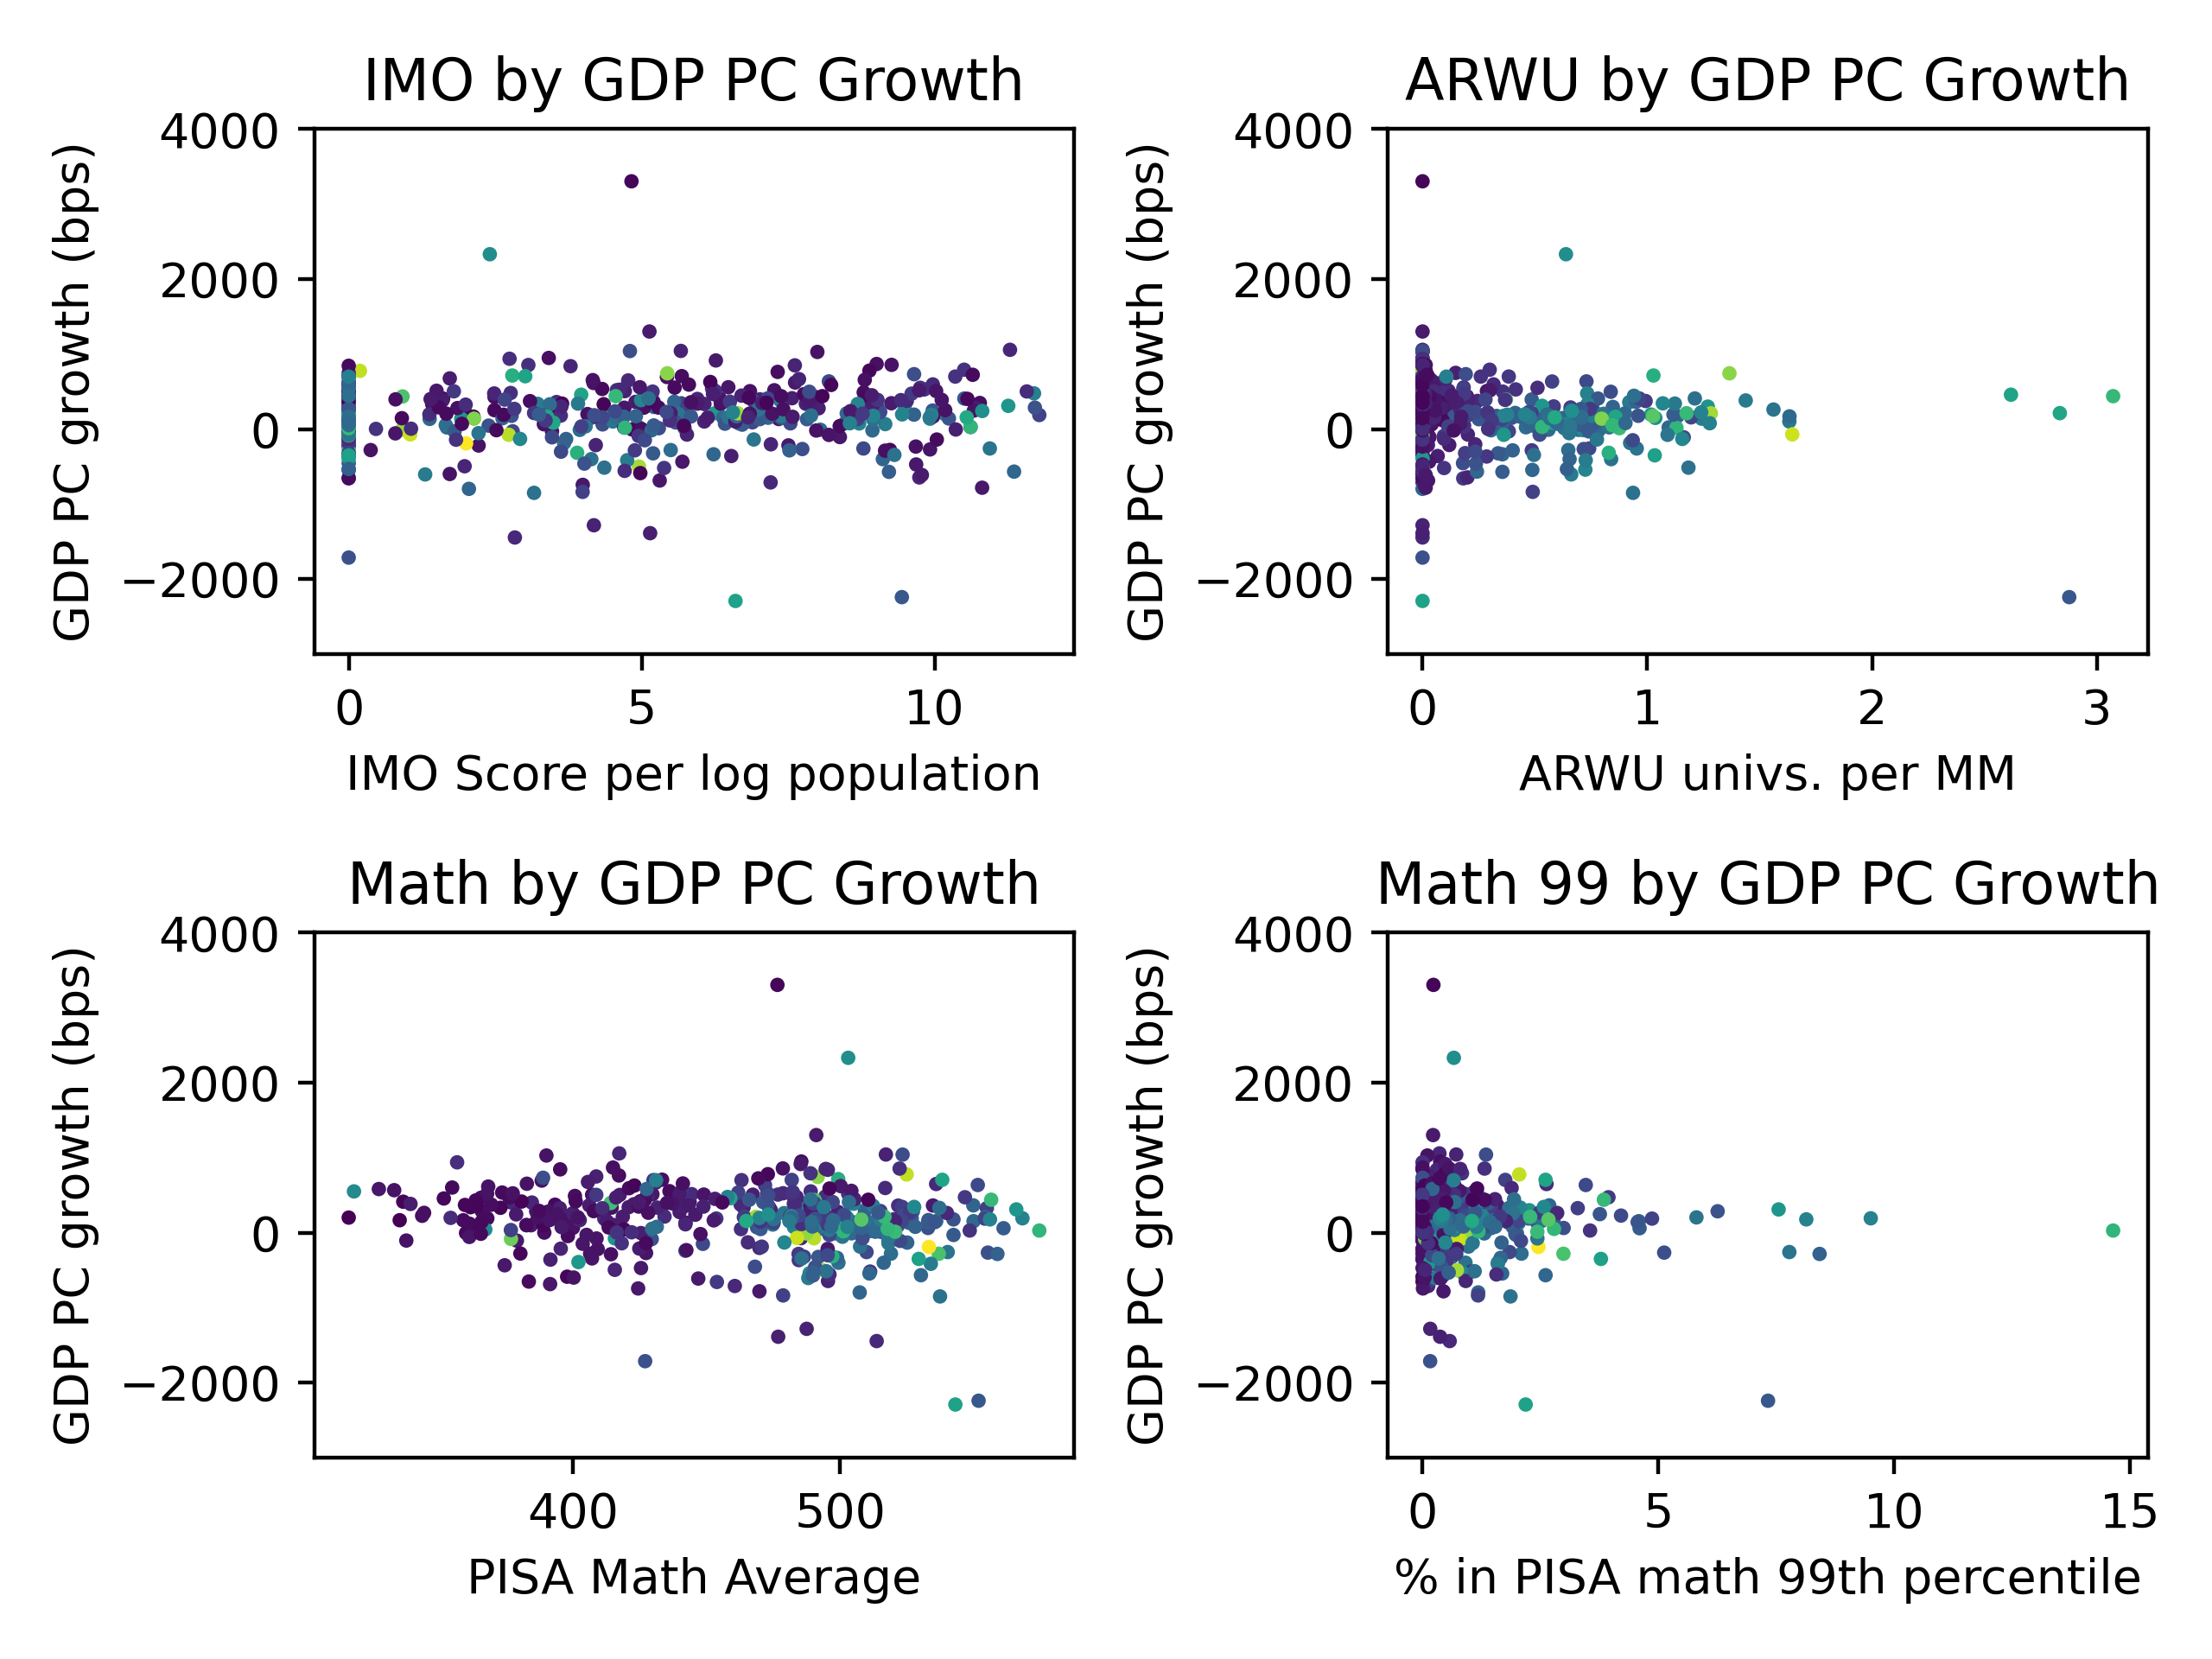
\includegraphics[width=0.6\textwidth]{../charts/relationships.png}
    \label{fig:relationships}
\end{figure}
By running specified regression models, we can examine the relationship while considering controls. It is clear from the picture above that we must consider this \textit{conditional} relationship. The regression coefficients on the elite orientation variables will indicate the size, direction, and significance of elite orientation condition on the controls included in the model. Comparing different model specifications will also let us examine the different assumptions made by each (e.g., time heterogeneity, within/between variation). The next section will discuss the interpretations and results with this in mind.
\section{Results and Interpretation}
\subsection{Panel Regressions}
We begin by estimating the panel regression specifications given above. The results are shown below in Table \ref{table:panel}\footnote{Full coefficient results available in appendix}.
\begin{table}[H] \centering
    \caption{Panel regression results (partial)}
    \label{table:panel}
    \resizebox{\linewidth}{!} {
        \begin{tabular}{@{\extracolsep{5pt}}lcccc}
            \\[-1.8ex]\hline
            \hline \\[-1.8ex]
            & \multicolumn{4}{c}{\textit{Dependent variable: GDP Per Capita Growth (bps)}} \
            \cr \cline{2-5}
            \\[-1.8ex] & \multicolumn{1}{c}{Model 1 (base)} & \multicolumn{1}{c}{Model 2 (with controls)} & \multicolumn{1}{c}{Model 3 (Time FE)} & \multicolumn{1}{c}{Model 4 (Time + Entity FE)}  \\
            \hline \\[-1.8ex]
             PISA Math in global P99 & -31.228$^{*}$ & -38.928$^{*}$ & -34.569$^{*}$ & -115.492$^{***}$ \\
            & (16.314) & (20.802) & (17.850) & (36.599) \\
             IMO score per log population & 10.674$^{*}$ & 4.924$^{}$ & 3.122$^{}$ & -11.158$^{}$ \\
            & (6.363) & (7.470) & (6.441) & (15.728) \\
             ARWU insitutions & -166.641$^{**}$ & -162.705$^{*}$ & -176.049$^{**}$ & -159.960$^{}$ \\
            & (68.800) & (86.871) & (72.281) & (112.884) \\
             Time Effects & No & No & Yes & Yes \\
             Fixed Effects & No & No & No & Yes \\
             Controls & No & Yes & Yes & Yes \\
             Entities & 89 & 89 & 89 & 89 \\
            \hline \\[-1.8ex]
             Observations & 440 & 440 & 440 & 440 \\
             $R^2$ & 0.037 & 0.077 & 0.374 & 0.553 \\
             Adjusted $R^2$ & 0.031 & 0.056 & 0.351 & 0.414 \\
             Residual Std. Error & 445.700 (df=436) & 439.888 (df=429) & 364.790 (df=423) & 346.511 (df=335) \\
             F Statistic & 5.616$^{***}$ (df=3; 436) & 3.589$^{***}$ (df=10; 429) & 15.813$^{***}$ (df=16; 423) & 3.983$^{***}$ (df=104; 335) \\
            \hline
            \hline \\[-1.8ex]
            \textit{Note:} & \multicolumn{4}{r}{$^{*}$p$<$0.1; $^{**}$p$<$0.05; $^{***}$p$<$0.01} \\
            \end{tabular}
    }
\end{table}

Model 1 includes only the elite orientation variables. We see a negative relationship between the share of students testing above the global 99th percentile and GDP per capita growth. At a coefficient of -31, this is significant magnitude-wise as it corresponds to a 31 bp reduction to GDP per capita growth for every percent of students in a country testing above the threshold (this variable has a mean of 0.94 and $\sigma=1.46$). With the average GDP per capita growth across the whole dataset being 169 bps, this is a noticeable effect. IMO test scores per log population in model 1 has a positive coefficient of 11, which given the mean of 4.72 and $\sigma=3.49$ is also a significant magnitude. The number of ARWU-ranked institutions per million population has a negative coefficient of -166 and is the most numerically significant since the mean of this variable is 0.26 and $\sigma=0.33$. An additional 0.1 ARWU-ranked institution per million population corresponds to a -16 bp reduction in GDP per capita growth.

Going to model 2 includes the set of control variables into the regression. We see that there is little change to the PISA math in global 99 and ARWU institutions variables. The coefficient of the IMO variable has decreased by half to 5. One possible explanation is the remaining $\rho=0.29$ correlation with population (also positively related to GDP per capita growth). Standard errors have increased for all coefficient estimates. This suggests that the elite orientation variables are measuring factors separate from the controls and thus average education level and wealth.

Including time fixed effects in model 3 further reduces the magnitude of the IMO score coefficient, but standard errors have decreased. The $R^2$ has increased significantly to 0.374, indicating that there are significant exogenous (to this model) effects on GDP per capita growth.

Finally, going to model 4, which include time and country fixed effects, has the largest effect on the coefficients and standard errors. However, the inclusion of country fixed effects means the regression is now estimating the within country effect rather than between countries. This is only valid if first, there is significant variation within the elite orientation variables within countries and second if we would expect such variation to be useful to interpretation.

Addressing the first assumption, we see that this is not the case. In table \ref{table:dummyreg} below, a regression model estimating each of the elite orientation variables using country dummies only show around 80\% of the variation in each variable coming purely from time-invariant country-level factors.

\begin{table}[!htbp] \centering
    \caption{Country dummy regression on elite orientation variables}
    \label{table:dummyreg}
    \resizebox{\linewidth}{!} {
    \begin{tabular}{@{\extracolsep{5pt}}lccc}
    \\[-1.8ex]\hline
    \hline \\[-1.8ex]
    \\[-1.8ex] & \multicolumn{1}{c}{in\_math99} & \multicolumn{1}{c}{imo\_total\_score} & \multicolumn{1}{c}{arwu\_ranked\_num}  \\
    \hline \\[-1.8ex]
    \hline \\[-1.8ex]
     Observations & 441 & 441 & 441 \\
     $R^2$ & 0.877 & 0.845 & 0.791 \\
     Adjusted $R^2$ & 0.846 & 0.807 & 0.738 \\
     Residual Std. Error & 0.573 (df=352) & 1.533 (df=352) & 0.171 (df=352) \\
     F Statistic & 28.437$^{***}$ (df=88; 352) & 21.875$^{***}$ (df=88; 352) & 15.096$^{***}$ (df=88; 352) \\
    \hline
    \hline \\[-1.8ex]
    \textit{Note:} & \multicolumn{3}{r}{$^{*}$p$<$0.1; $^{**}$p$<$0.05; $^{***}$p$<$0.01} \\
    \end{tabular}
    }
\end{table}
The first assumption is thus violated when interpreting model 4. This paper uses the elite orientation variables as proxies for cultural and institutional factors which are unlikely to have varied significantly in the period of 2003-2022, especially as the PISA countries tend to be wealthier and more stable. Thus, the second assumption in interpreting model 4 is also violated. However, this supports the premise of this paper that the elite orientation variables are capturing these cultural and institutional factors separate from average academic achievement.

Due to data availability, this panel is also imbalanced, which will potentially bias the coefficients as some countries are given more weight (primarily due to which countries are tested by PISA). A summary of the panel is given below in table \ref{table:panel-stats}.
\begin{table}[H]
    \caption{Panel statistics}
    \label{table:panel-stats}
    \centering
    \begin{tabular}{llll}
    Entities     & 89     &  &   \\
    Avg Obs      & 4.9438 &  &   \\
    Min Obs      & 1      &  &   \\
    Max Obs      & 7      &  &   \\
                 &        &  &   \\
    Time periods & 7      &  &   \\
    Avg Obs      & 62.857 &  &   \\
    Min Obs      & 40     &  &   \\
    Max Obs      & 76     &  &  
    \end{tabular}
\end{table}

\subsection{Yearly Regressions}
The results from the earlier panel regressions assume that the relationship between the elite orientation variables and growth is static through time. Whether this is true can be tested by regressing each year separately and comparing the results in table \ref{table:yearly}\footnote{Full regression results available in appendix}.
\begin{table}[H] \centering
    \caption{Yearly regression results (partial)}
    \label{table:yearly}
    \resizebox{\linewidth}{!} {
        \begin{tabular}{@{\extracolsep{1pt}}lcccccccc}
            \\[-1.8ex]\hline
            \hline \\[-1.8ex]
            & \multicolumn{8}{c}{\textit{Dependent variable: GDP Per Capita Growth (bps)}} \
            \cr \cline{2-9}
            \\[-1.8ex] & \multicolumn{1}{c}{2003} & \multicolumn{1}{c}{2006} & \multicolumn{1}{c}{2009} & \multicolumn{1}{c}{2012} & \multicolumn{1}{c}{2015} & \multicolumn{1}{c}{2018} & \multicolumn{1}{c}{2022} & \multicolumn{1}{c}{Panel FE}  \\
            \hline \\[-1.8ex]
             PISA Math in global P99 & -52.490$^{}$ & -193.475$^{**}$ & 154.062$^{**}$ & 16.575$^{}$ & -34.309$^{}$ & 3.769$^{}$ & -69.681$^{**}$ & -115.492$^{***}$ \\
            & (48.524) & (84.559) & (62.680) & (36.365) & (76.140) & (27.106) & (27.702) & (36.599) \\
             IMO score per log population & 4.478$^{}$ & -9.112$^{}$ & 14.038$^{}$ & 7.368$^{}$ & -16.622$^{}$ & 2.193$^{}$ & -0.174$^{}$ & -11.158$^{}$ \\
            & (17.327) & (20.741) & (17.012) & (13.983) & (27.567) & (7.722) & (13.474) & (15.728) \\
             ARWU insitutions & -300.038$^{**}$ & -454.401$^{***}$ & 136.623$^{}$ & -344.990$^{**}$ & 289.270$^{}$ & 61.220$^{}$ & -829.105$^{***}$ & -159.960$^{}$ \\
            & (111.479) & (167.497) & (188.401) & (133.886) & (270.034) & (125.503) & (206.280) & (112.884) \\
            Controls & Yes & Yes & Yes & Yes & Yes & Yes & Yes & Yes \\
            \hline \\[-1.8ex]
             Observations & 40 & 56 & 69 & 61 & 65 & 73 & 76 & 440 \\
             $R^2$ & 0.675 & 0.499 & 0.264 & 0.302 & 0.100 & 0.294 & 0.417 & 0.553 \\
             Adjusted $R^2$ & 0.562 & 0.387 & 0.137 & 0.162 & -0.067 & 0.180 & 0.327 & 0.414 \\
             Residual Std. Error & 179.479 (df=29) & 365.156 (df=45) & 402.134 (df=58) & 254.369 (df=50) & 490.971 (df=54) & 180.728 (df=62) & 335.236 (df=65) & 346.511 (df=335) \\
             F Statistic & 6.011$^{***}$ (df=10; 29) & 4.479$^{***}$ (df=10; 45) & 2.075$^{**}$ (df=10; 58) & 2.158$^{**}$ (df=10; 50) & 0.598$^{}$ (df=10; 54) & 2.581$^{**}$ (df=10; 62) & 4.649$^{***}$ (df=10; 65) & 3.983$^{***}$ (df=104; 335) \\
            \hline
            \hline \\[-1.8ex]
            \textit{Note:} & \multicolumn{8}{r}{$^{*}$p$<$0.1; $^{**}$p$<$0.05; $^{***}$p$<$0.01} \\
            \end{tabular}
    }
    \end{table}

From table \ref{table:yearly}, we see that there is significant year-to-year change in the magnitude and direction of the elite orientation coefficients. Over the 7 distinct years, the $R^2$ also varies significantly, which suggests that exogenous changes in the world affect the explanatory power of the controls and elite orientation variables.

In 2009, we can see that the coefficients direction has been inverted relative to 2006 and 2012. This is likely due to the impact of the 2008 Financial Crisis on the global economy. For instance, Asian countries and regions such as Singapore and Hong Kong perform highly in PISA tests but were less affected by 2008. This suggests that omitted variable bias may be a serious problem when looking at individual years.

Taken together, there is no clear statistical relationship between the elite orientation variables and economic growth in the yearly regressions either. Out of the three variables, the ARWU variable has the most consistent relationship (negative, mostly) with GDP per capita growth. Universities are slow-moving institutions, so this makes sense.

\subsection{Expanding the dataset by removing PISA variables}
The high standard errors for the regression and limited data suggest that expanding the dataset may provide additional color.
The results are described in table \ref{table:expanded}.
\begin{table}[H] \centering
    \caption{Expanded regression results}
    \label{table:expanded}
    \resizebox{\linewidth}{!} {
    \begin{tabular}{@{\extracolsep{5pt}}lccccc}
    \\[-1.8ex]\hline
    \hline \\[-1.8ex]
    & \multicolumn{5}{c}{\textit{Dependent variable: GDP per capita growth}} \
    \cr \cline{2-6}
    \\[-1.8ex] & \multicolumn{1}{c}{Model 3 (PISA)} & \multicolumn{1}{c}{PISA countries exc. math} & \multicolumn{1}{c}{PISA years} & \multicolumn{1}{c}{All years} & \multicolumn{1}{c}{All years, FE}  \\
    \hline \\[-1.8ex]
    IMO score per log population & 3.122$^{}$ & -0.460$^{}$ & 3.647$^{}$ & 17.239$^{***}$ & -9.490$^{}$ \\
    & (6.441) & (5.913) & (6.516) & (3.546) & (8.562) \\
    ARWU insitutions & -176.049$^{**}$ & -196.841$^{***}$ & -183.403$^{**}$ & -191.701$^{***}$ & -342.927$^{***}$ \\
    & (72.281) & (71.171) & (82.042) & (44.185) & (87.248) \\
    GDP per capita & -0.001$^{}$ & -0.002$^{**}$ & -0.001$^{*}$ & -0.001$^{*}$ & 0.008$^{***}$ \\
    & (0.001) & (0.001) & (0.001) & (0.000) & (0.002) \\
    Primary School Completion Rate & -6.467$^{*}$ & -5.609$^{*}$ & 1.830$^{}$ & 1.072$^{}$ & 6.805$^{***}$ \\
    & (3.586) & (3.338) & (1.560) & (0.839) & (1.228) \\
    Lower Sec. Completion Rate & -0.953$^{}$ & -0.862$^{}$ & 1.472$^{}$ & 1.982$^{*}$ & 4.331$^{***}$ \\
    & (2.958) & (2.965) & (2.253) & (1.202) & (1.453) \\
    Upper Sec. Completion Rate & 5.721$^{**}$ & 5.837$^{**}$ & -0.448$^{}$ & -1.451$^{}$ & -4.847$^{***}$ \\
    & (2.375) & (2.373) & (2.071) & (1.110) & (1.387) \\
    Democracy Rating & -5.350$^{}$ & -2.178$^{}$ & -17.044$^{**}$ & -10.445$^{**}$ & 102.359$^{***}$ \\
    & (14.344) & (13.998) & (7.517) & (4.069) & (24.736) \\
    Population & -0.000$^{}$ & -0.000$^{}$ & 0.000$^{**}$ & 0.000$^{***}$ & -0.000$^{}$ \\
    & (0.000) & (0.000) & (0.000) & (0.000) & (0.000) \\
    Time Effects & Yes & Yes & Yes & Yes & Yes \\
    Fixed Effects & No & No & No & No & Yes \\
    Entities & 49 & 49 & 213 & 213 & 213 \\
    \hline \\[-1.8ex]
    Observations & 440 & 440 & 1424 & 4094 & 4094 \\
    $R^2$ & 0.374 & 0.368 & 0.103 & 0.188 & 0.294 \\
    Adjusted $R^2$ & 0.351 & 0.347 & 0.094 & 0.183 & 0.250 \\
    Residual Std. Error & 364.790 (df=423) & 365.736 (df=425) & 567.654 (df=1409) & 518.050 (df=4066) & 496.134 (df=3853) \\
    F Statistic & 15.813$^{***}$ (df=16; 423) & 17.680$^{***}$ (df=14; 425) & 11.537$^{***}$ (df=14; 1409) & 34.906$^{***}$ (df=27; 4066) & 6.699$^{***}$ (df=240; 3853) \\
    \hline
    \hline \\[-1.8ex]
    \textit{Note:} & \multicolumn{5}{r}{$^{*}$p$<$0.1; $^{**}$p$<$0.05; $^{***}$p$<$0.01} \\
    \end{tabular}
    }
    \end{table}
Moving from model 3 to the same data but excluding PISA variables (mean and math 99) we can see that there is some omitted variable bias with the IMO coefficient decreasing significantly and the ARWU institution variable decreasing (although less) as well.

Expanding the data to first all countries in the same PISA years, and then to all years, reduces the standard error significantly of estimates. The “All years” and “All years, FE” models correspond to model 3 and 4 respectively. The ARWU coefficient has changed the least, but the IMO coefficient has seen a significant decrease in standard error and increase in magnitude to 20. Both elite orientation variables are now statistically significant at the 1\% level. Including country-level fixed effects again introduces large changes that reflect that the elite orientation variables tend to be stable within countries.

Although there is a clear omitted variable bias concern with this approach, it does suggest that the relationships are consistent directionally and roughly in magnitude.
\subsection{Direction of relationship}
While there exist differences between years and regression specifications, the PISA math in global 99th percentile and ARWU variables have a mostly negative relationship with GDP per capita growth, while the IMO score coefficients tend to be positive. From a theoretical perspective, it is not clear why having more high-performing math students and top-ranked universities would contribute negatively to economic growth.

One possible explanation of this is that the PISA math in global 99th percentile and ARWU variables display a very similar non-linear relationship with GDP per capita. As this relationship is not linear, controlling for GDP per capita is insufficient. The inclusion of these variables may instead of allowing for non-linear convergence dynamics in economic growth, which is a possible explanation for why the coefficients are negative.

\begin{figure}[H]
    \caption{Relationships of variables with GDP per capita}
    \centering
    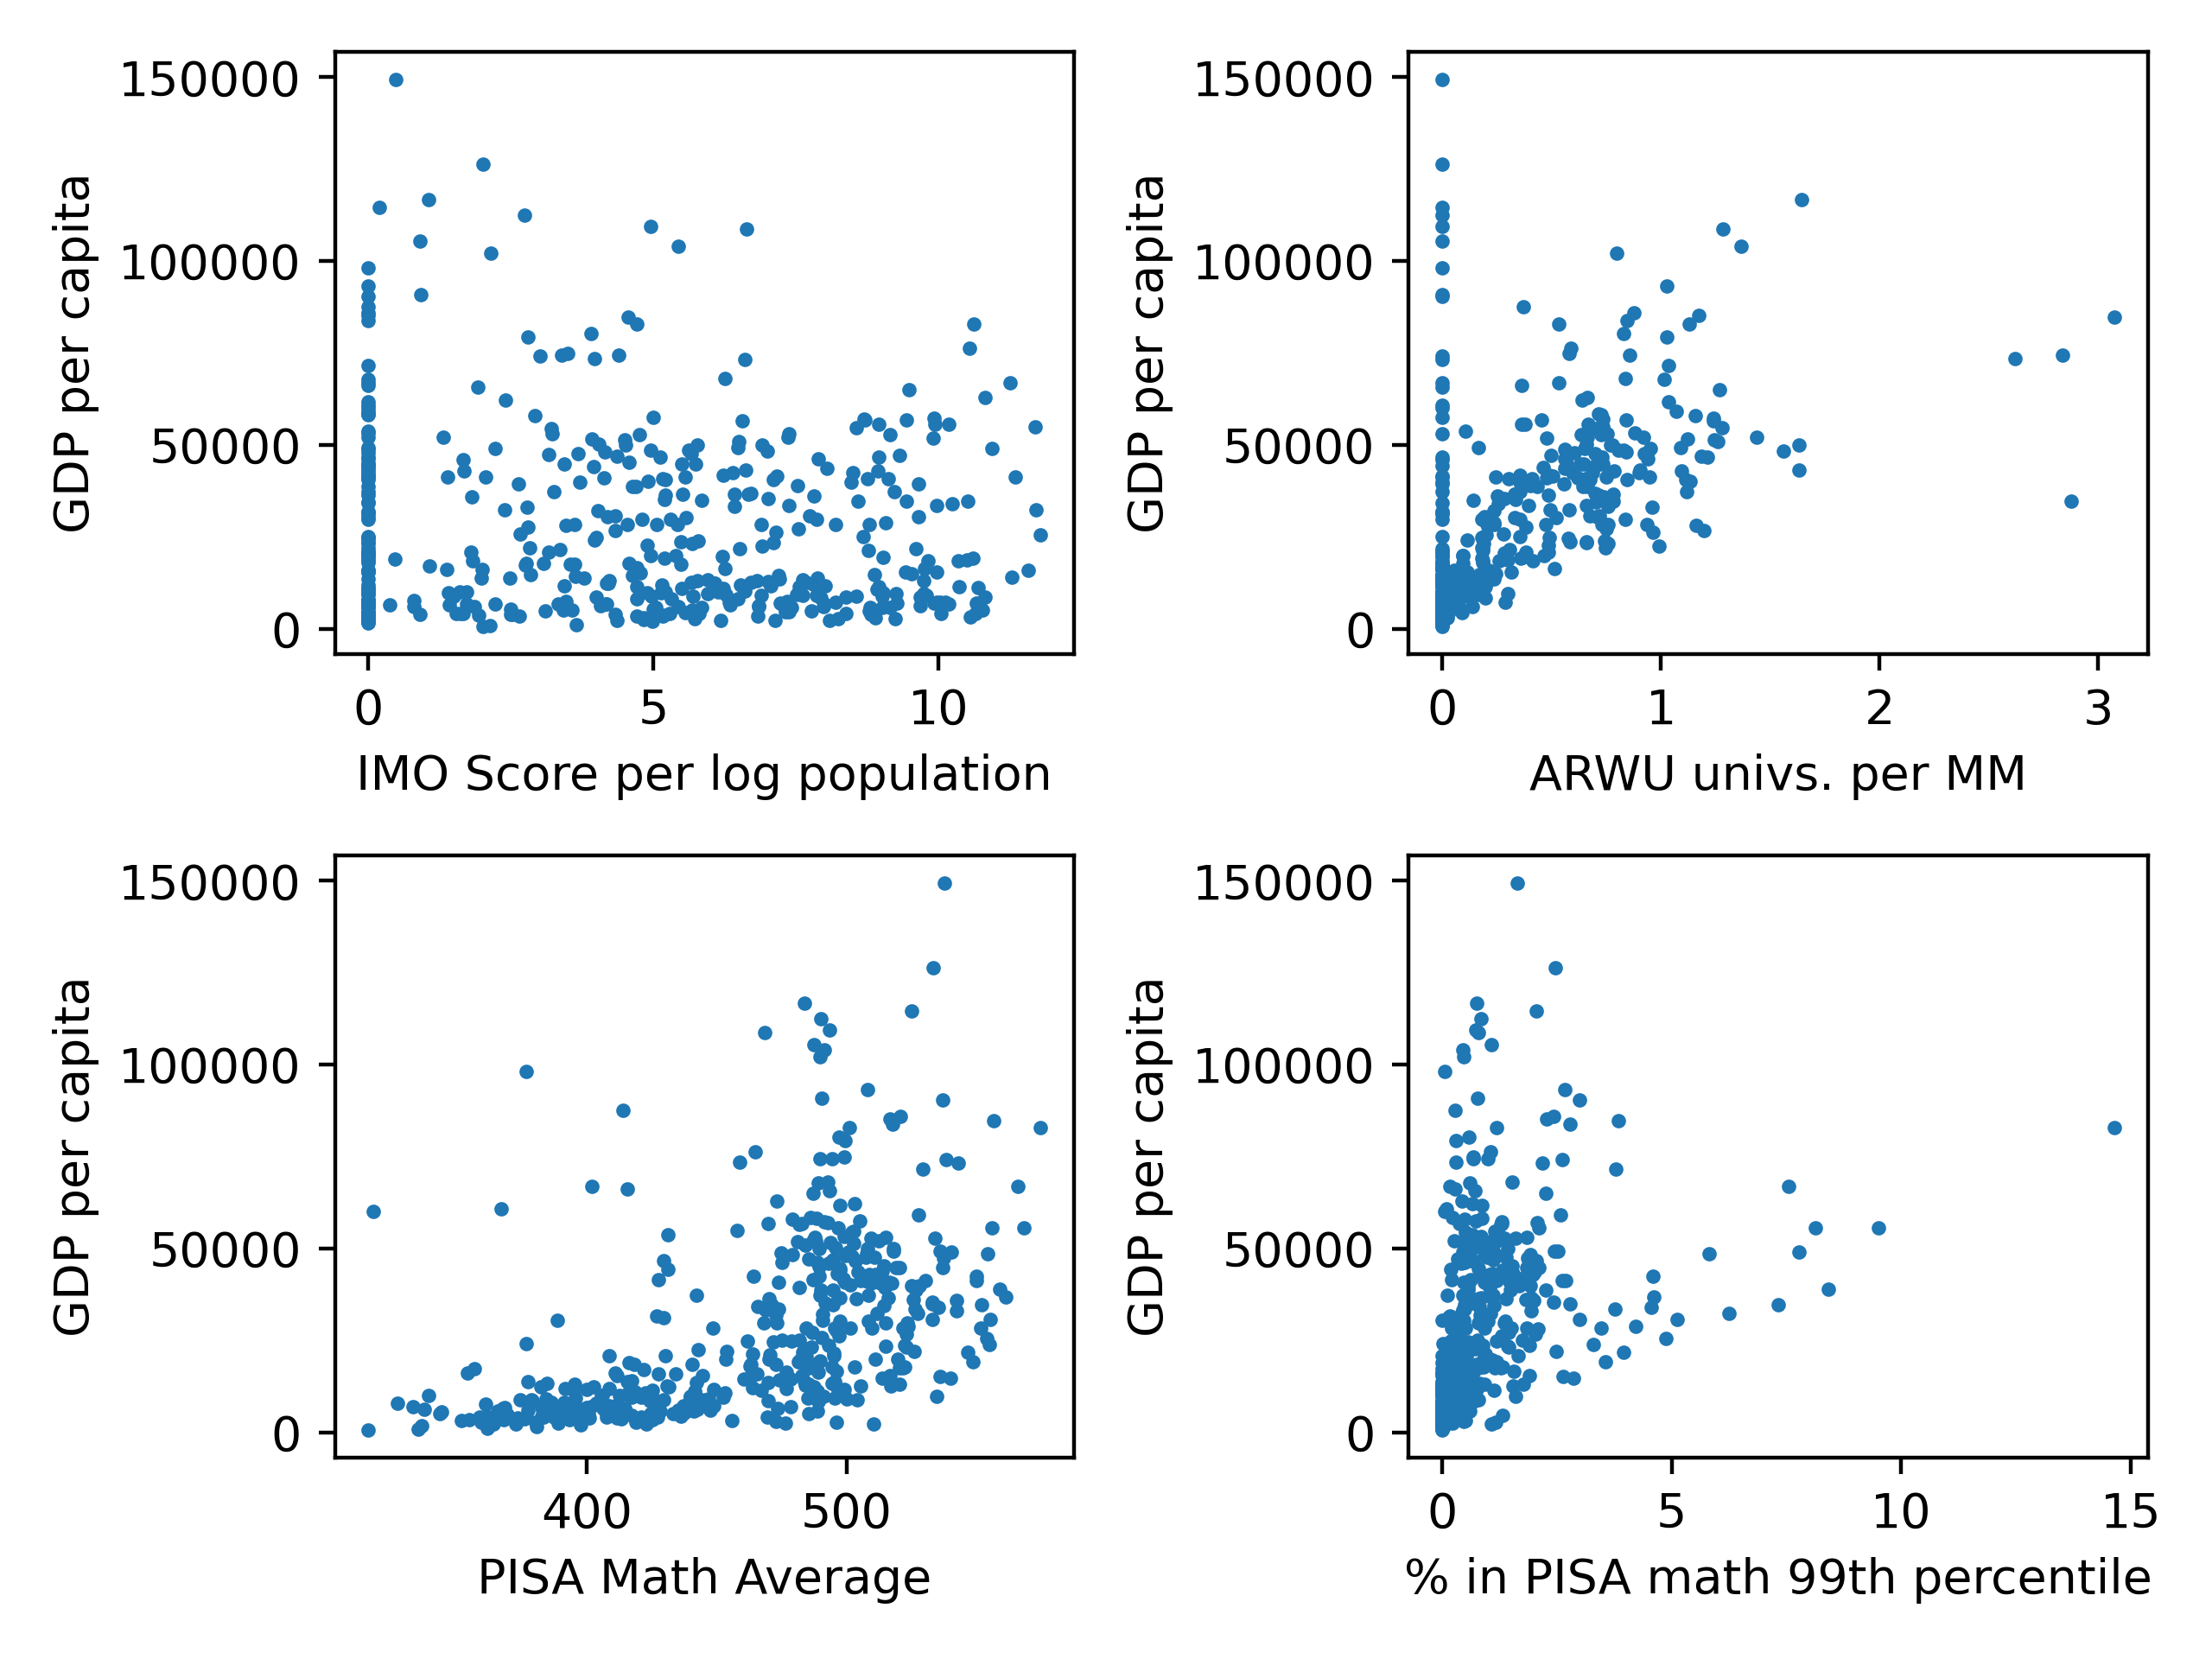
\includegraphics[width=0.6\textwidth]{../charts/relationships-gdp-pc.png}
    \label{fig:relationships-gdppc}
\end{figure}


\begin{figure}[H]
    \caption{Total scatter plot}
    \centering
    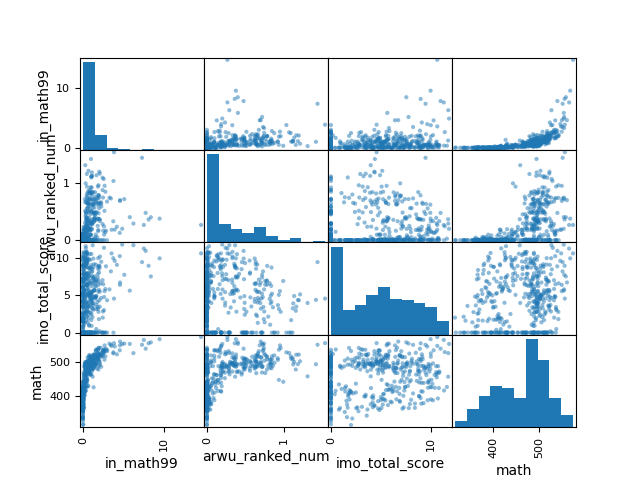
\includegraphics[width=0.6\textwidth]{../build/total.png}
    \label{fig:relationships-all}
\end{figure}

PISA math in 99 and ARWU institution variables also display a strong non-linear relationship with mean PISA math scores (see figure \ref{fig:relationships-gdppc} and \ref{fig:relationships-all}).

However, IMO scores measure a different set of latent factors than PISA math 99 and ARWU variables. Generally, IMO scores display a very different relationship with the other variables to suggest this. The correlation with GDP per capita is very low and the strength of correlation with PISA math 99 and ARWU variables is also low.

It may be the case that higher ARWU rankings and top math performer shares are areas where countries tend to invest in as they develop. While a higher proportion of high-performing students may indicate something about academic culture and incentives, IMO scores provide a strong indication of such as it is less likely to be tied to overall economic development. Empirically this appears true when looking at the correlations with GDP per capita.

Returning to the effective participating talent pool theory, IMO performance is thus a better instrument for measuring the “motivation” portion of the pool, as there are little rewards baked into the actual Olympiad for those not selected. Any remaining incentive must thus come from within the country (e.g., university admissions, getting into Jane Street, status). These incentives can be grouped under the cultural and institutional/structural elite orientation of an education system. The above is likely to be true as it is difficult for a country to do well without a large pool of students willing to practice and compete.

This suggests that IMO performance may be the best proxy out of the variables and is likely measuring something different from the other two variables.

\subsection{Does IMO performance measure something else?}
To explore whether IMO performance indeed captures a different set of unobservable factors (the cultural and institutional/structural elite orientation of an education system) compared to PISA math 99 share and ARWU institution count. Principle Components Analysis (PCA) may help analyze this by projecting the 3 variables onto 2 orthogonal vectors.

\section{Limitations}
The inconsistent results between different model specifications and high standard errors suggest that there are significant concerns with this study. I outline several key concerns below and discuss their severity.

\subsection{Imputation Problems}
As around 75\% of the school completion rates in the dataset are imputed with XGBoost, there are concerns that this may introduce bias into the dataset. First, tree-based models are prone to overfitting, so the imputed data may bias the regression. Second, the fitted values have unknown errors (as many countries never had any completion data at all). To help reduce the first concern, the training data is a superset of the regression data and includes many more countries and years. Cross validation is also used to reduce overfitting.
\pagebreak
\nocite{*}
\printbibliography
\end{document}
